\documentclass[10pt,journal]{IEEEtran}
\usepackage[T1]{fontenc}
\usepackage{amsmath,amssymb,amsfonts,booktabs,graphicx,multirow,url,cite,xcolor}
\usepackage{tikz}
\usetikzlibrary{arrows.meta,positioning}
\usepackage[colorlinks=true,linkcolor=blue!65!black,citecolor=blue!65!black,urlcolor=blue!65!black]{hyperref}

\setlength{\tabcolsep}{3.8pt}
\renewcommand{\arraystretch}{1.10}
\setlength{\emergencystretch}{2em}
\tolerance=1000
\setcounter{topnumber}{4}
\setcounter{dbltopnumber}{4}
\setcounter{totalnumber}{6}
\renewcommand{\topfraction}{0.95}
\renewcommand{\dbltopfraction}{0.95}
\renewcommand{\textfraction}{0.05}
\renewcommand{\floatpagefraction}{0.88}
\renewcommand{\dblfloatpagefraction}{0.88}

\markboth{ARXIV PREPRINT}{TIWATER: EVIDENCESCENE: OBSERVABILITY-CONDITIONED POSE TRACKING AND REVISABLE 3D SCENE RECONSTRUCTION}

\title{EvidenceScene: Observability-Conditioned Pose\\ Tracking and Revisable 3D Scene Reconstruction\\ for Robot Manipulation}
\author{Tiwater\\
{\normalsize\href{mailto:research@tiwater.com}{\texttt{research@tiwater.com}}}%
\thanks{Tiwater (e-mail: \href{mailto:research@tiwater.com}{\texttt{research@tiwater.com}}). Project page: \url{https://tiwater.github.io/evidencescene/}.}}

\begin{document}
\sloppy
\maketitle

\begin{abstract}\normalfont
Model-free 6D pose tracking and online surface reconstruction from RGB-D video remain brittle when depth support is sparse, objects self-occlude, or local geometry is degenerate. A common assumption is that returning more poses, or lowering an internal optimization residual, yields a more reliable reconstruction. We show that this assumption fails. Across a 31-framework audit, repairing two Point2Pose implementation defects ($F=F_1+F_2$) on Laval Cookiejar raises pose availability from $207$ to $239/295$ frames and failure-inclusive ADD AUC from $0.574$ to $0.635$, yet reduces $20\,\mathrm{mm}$ origin successes from $136$ to $120$ and drops Frame-150 $10\,\mathrm{mm}$ surface coverage $C_{10}$ from $76.82\%$ to $61.79\%$ ($64.85\%$ on a fixed $16$-keyframe set). We trace this availability--surface paradox to three coupled mechanisms: unanchored $\mathrm{SE}(3)$ gauge drift in disconnected graph components, nuisance-coupled rank deficiency after landmark elimination, and pose-version desynchronization between graph revisions and fused surfaces. We present EvidenceScene, a standalone, causal (no future-frame) framework evaluated across three evidence tracks: (i) an offline mechanism audit on Point2Pose isolating prior-connected admission ($G$), marginal Schur rank gating ($R$), immutable feature-birth ledgers ($M$), and surface-history transactions ($S$, including $R+S$ and open- vs.\ closed-loop TSDF refinement feedback); (ii) deterministic native engineering on our BundleTrack pose owner and \texttt{RevisableSurfelMap} surface owner, where stable-winner CUDA RANSAC and exact $\mathrm{SE}(3)$ inverse transfer raise Clock/Cookiejar strict successes from $135/107$ to $191/136$ ($30.24\,\mathrm{ms}$ single-stage tracker median on YCBInEOAT), guarded \texttt{NO\_BA} retirement saves $928.4$--$1{,}994.0\,\mathrm{MiB}$ RSS with byte-identical outputs across $18$ wrist-camera replays ($\Delta\text{AUC}\le 0.0004$ on Laval local BA), and an array-native \texttt{support10/coarse12mm} selector raises $1{,}500$-point measured-surfel $C_{10}$ from $40.57\%/52.34\%$ to $85.10\%/85.05\%$ ($R_{95}$ $53.12/31.88\to 13.12/12.47\,\mathrm{mm}$) at a bounded precision trade-off ($P_{10}$ $100.00\%/84.13\%\to 99.00\%/81.73\%$, $F_{95}$ $5.27/12.54\to 7.33/13.17\,\mathrm{mm}$) while accelerating $60\mathrm{k}$-point update ($73.00\to 1.05\,\mathrm{ms}$, $69.8\times$), snapshot ($20.48\to 0.22\,\mathrm{ms}$, $93.0\times$), and selection ($15.52\to 1.05\,\mathrm{ms}$, $14.8\times$; $45.8\times$ 3-kernel geomean, $8.65\times$ across all 7 \texttt{kernel-v1} workloads); and (iii) a frozen $2\times 2$ factorial ($\text{Gate}\times S$) on a single unified output branch across three independent RGB-D sequences ($87$ post-initial frames), where joint gating and birth-indexed surface revision prevent degenerate surface corruption ($P_{10}(t_{\mathrm{deg}})$ $77.80\%\to 86.53\%$, $F_{95}$ $24.52\to 14.77\,\mathrm{mm}$) and reach terminal $P_{10}/C_{10}=100.00\%/99.39\%$ ($F_{95}/R_{95}=4.48/3.67\,\mathrm{mm}$, retained ADD AUC $0.9871$, committed mean ADD $1.03\,\mathrm{mm}$ vs.\ $8.27\,\mathrm{mm}$ un-gated). Finally, bit-exact runtime adapters overlap SAM~2 GPU waits with CPU preparation and use $O(\text{runs})$ RLE arithmetic, cutting warm 4-camera HTTP endpoint replay $p_{50}/p_{95}$ from $155.33/219.06\,\mathrm{ms}$ to $127.80/153.40\,\mathrm{ms}$ at $499/499$ parity, while live physical site acceptance remains $0/6$.
\end{abstract}

\begin{IEEEkeywords}\normalfont
EvidenceScene, evidence-constrained 3D scene reconstruction, RGB-D object tracking, revisable surface reconstruction, factor-graph observability, degenerate geometry, robot manipulation, bit-exact runtime optimization, reproducibility.
\end{IEEEkeywords}

\section{Introduction}
\label{sec:intro}

\IEEEPARstart{O}{nline} 6-DoF object pose tracking and 3D surface reconstruction from onboard RGB-D streams provide essential spatial awareness for remote humanoid teleoperation and bimanual manipulation~\cite{bundletrack,bundlesdf,point2pose}. Without pre-loaded CAD models, a manipulation perception system must initialize an object coordinate gauge from the first segmented RGB-D observation, track relative rigid motion across occlusions and depth dropouts, and accumulate a geometrically trustworthy 3D surface for operator guidance.

A common assumption in model-free tracking benchmarks is that returning a higher fraction of non-lost poses---or achieving a lower internal optimization residual---naturally yields a more reliable 3D reconstruction. Our empirical investigation refutes this assumption. Under sparse depth support, self-occlusion, or locally degenerate geometry, long-horizon 2D point trajectories and dense correspondences frequently constrain only a subspace of the joint pose-landmark state. Admitting unconstrained or unanchored updates into persistent object maps and volumetric/surfel surfaces can corrupt previously verified geometry even while increasing frame-level pose availability.

To prevent implementation artifacts from being conflated with algorithmic gains, we introduce \textbf{EvidenceScene} (\emph{Observability-Conditioned 3D Scene Reconstruction for Robot Manipulation}) and strictly distinguish three methodological entities and three evaluation tracks throughout this study: (1) the upstream BundleTrack algorithm~\cite{bundletrack} (pinned to \texttt{ffa67d425240}), (2) the upstream Point2Pose point-trajectory tracker and TSDF reconstructor~\cite{point2pose} (pinned to \texttt{51856226610d}), and (3) our proposed \textbf{EvidenceScene} framework. Because the live teleoperation stack uses native BundleTrack + \texttt{RevisableSurfelMap} while upstream Point2Pose uses GTSAM + \texttt{SDFBuilder}, we report: (a) an offline mechanism audit on Point2Pose ($F,G,R,M,S$, including $R+S$ and open- vs.\ closed-loop TSDF feedback), (b) native determinism, memory, and surface-selection repairs on the BundleTrack + \texttt{RevisableSurfelMap} branch, and (c) a frozen $2\times 2$ factorial ($\text{Observability Gate}\times\text{Surface Revision }S$) on a single unified output branch across three independent RGB-D sequences. Throughout, \emph{causal} means that an estimate at time $t$ is a function of observations up to $t$; no future frame is consulted.

\textbf{Evidence scope.} Public YCBInEOAT and Laval results are development audits on recordings available during method design; pose scores use reference masks and Frame-0 gauge alignment, and all benchmark surface scores ($P_{10},C_{10},F_{95},R_{95}$) evaluate \emph{measured sensor surfels only} ($\texttt{is\_prior}=\texttt{False}$, excluding Stage-0 generative priors) against a CAD or sampled-model reference. Generalization of the unified $\text{Gate}\times S$ mechanism is evaluated under a frozen configuration across three independent multi-phase RGB-D sequences ($87$ post-initial frames), whereas live physical site acceptance remains $0/6$ passed (\texttt{gate\_passed=false}).

Our contributions are fourfold:
\begin{enumerate}
    \item \textbf{Failure Mechanism Audit and Closed-Loop TSDF Feedback Attribution (Sections~\ref{sec:problem}--\ref{sec:method}, \ref{sec:experiments}-A/B):} We formalize three coupled failure modes in long-horizon RGB-D tracking and fusion: (i) temporal attribution ($F_1$) and solver-return inconsistency ($F_2$), showing on Cookiejar that $79.6\%$ of the Frame-150 coverage drop ($76.82\%\to 61.79\%$) stems from unanchored graph drift on the $16$ shared keyframes triggered by $F_2$; (ii) unanchored $\mathrm{SE}(3)$ gauge drift and nuisance-coupled rank deficiency after orthogonal left-null-space landmark elimination $\bar{\mathbf{A}}_x=(\mathbf{I}-\mathbf{A}_y\mathbf{A}_y^+)\mathbf{A}_x$, with a complete numerical specification of the multi-scale Schur rank gate ($R$); and (iii) pose-version desynchronization in surface fusion ($S$), explaining why $S$ alters online poses in Point2Pose via trilinear \texttt{SDFBuilder} pose-refinement queries and evaluating both open-loop (fixed-pose) and closed-loop ($G,R,M\times S$) surface metrics.
    \item \textbf{Unified-Branch $2\times 2$ Factorial and Native BundleTrack Governance (Sections~\ref{sec:native_bt}, \ref{sec:experiments}-C):} On a single unified output branch with frozen thresholds across three independent RGB-D sequences, we execute a $2\times 2$ factorial ($\text{Gate ON/OFF}\times S\text{ ON/OFF}$) with per-frame commit ledgers and time-varying $P_{10}(t),C_{10}(t),F_{95}(t),R_{95}(t)$, demonstrating that gating protects already-reconstructed geometry during degeneracy while $S$ removes pre-BA keyframe drift ($P_{10}/C_{10}=100.00\%/99.39\%$, $F_{95}/R_{95}=4.48/3.67\,\mathrm{mm}$). On native BundleTrack, deterministic CUDA RANSAC and exact $\mathrm{SE}(3)$ inverse transfer raise Clock/Jar strict hits from $135/107$ to $191/136$, and guarded \texttt{NO\_BA} retirement reclaims $928.4$--$1{,}994.0\,\mathrm{MiB}$ RSS with byte-identical outputs across $18$ wrist replays.
    \item \textbf{Lineage-Audited \texttt{RevisableSurfelMap} and Columnar Budget Selection (Section~\ref{sec:surface_selection}):} By tracing $1{,}512{,}357$ surfel contributions to $1{,}960{,}512$ source pixels and continuous mesh rays, we separate pose-induced surface tails from raw boundary measurements. Unlike volumetric de-integration in BundleFusion~\cite{bundlefusion}, \texttt{RevisableSurfelMap} indexes pre-quantized object-frame voxel centroids by birth keyframe to execute $O(|V_{\mathrm{rev}}|)$ signed delta revisions ($2.97\,\mathrm{ms}$ vs.\ $7.49\,\mathrm{ms}$ full-history re-integration at $60\mathrm{k}$ points with bit-exact parity), while \texttt{support10/coarse12mm} raises $1{,}500$-point $C_{10}$ from $40.57\%/52.34\%$ to $85.10\%/85.05\%$ ($45.8\times$ 3-kernel geomean; $8.65\times$ across all 7 \texttt{kernel-v1} workloads).
    \item \textbf{31-Framework Context and Bit-Exact Runtime Execution Optimization (Sections~\ref{sec:runtime_opt}--\ref{sec:experiments}-D, Appendix~\ref{app:landscape}):} Across a 31-framework audit (Table~\ref{tab:framework_audit}), we benchmark foundation depth models, pointmap transformers, segmenters, trackers, and matchers on identical registered inputs, and introduce \texttt{SAM2GpuWindowOverlapScope} and \texttt{RequestEvidenceDeduplicationScope} ($O(\text{runs})$ exact integer RLE arithmetic, cross-stage surface/medoid reuse, BLAS-screened coplanar RANSAC, and request-boundary cyclic GC control), cutting warm 4-camera HTTP endpoint replay latency by $27.6\%$ ($176.40\to 127.80\,\mathrm{ms}$ $p_{50}$, $219.06\to 153.40\,\mathrm{ms}$ $p_{95}$) with $100\%$ bit-exact parity.
\end{enumerate}

\section{Related Work and Architectural Landscape}
\label{sec:related}

\textbf{Model-Free 6-DoF Pose Tracking, Point Tracking, and Feature Matching:} Model-free RGB-D trackers estimate camera-local object motion from an initial segmented frame for manipulation tasks~\cite{zhao2023learning,chi2023diffusion}. BundleTrack~\cite{bundletrack} combines pairwise feature matching with keyframe pose-graph optimization over sparse 3D correspondences and dense point-to-plane residuals. BundleSDF~\cite{bundlesdf} jointly optimizes a keyframe pose graph and a neural implicit signed distance field, whereas FoundationPose~\cite{foundationpose} and Any6D~\cite{lee2025any6d} unify CAD-based and few-view reference-assisted pose estimation, alongside iterative, Gaussian Splatting~\cite{kerbl20233dgs}, and KV-cache trackers such as BIT~\cite{song2025bit}, 6DOPE-GS~\cite{jin20256dopegs}, and KV-Tracker~\cite{elich2026kvtracker}. Point2Pose~\cite{point2pose} introduces long-horizon 2D point tracking (Online BootsTAPIR~\cite{bootstap}, alongside TAPNext++~\cite{zholus2025tapnext} and CoTracker3~\cite{karaev2024cotracker3}) across occlusions, lifting 2D tracks to 3D observations for multi-hypothesis SVD-RANSAC~\cite{fischler1981ransac,umeyama1991least} registration, GTSAM~\cite{gtsam} / iSAM2~\cite{kaess2012isam2} Levenberg-Marquardt pose-landmark graph optimization, and incremental TSDF fusion. While Point2Pose's point identity persistence, multi-object query management, and graph/TSDF architecture are established upstream contributions, we show that its unguarded graph commits and closed-loop TSDF pose-refinement coupling can degrade surface fidelity when 2D tracks lack well-distributed 3D depth support. In parallel, replacing detector-free LoFTR~\cite{loftr} or dense RoMa~\cite{edstedt2024roma} with faster matchers such as EfficientLoFTR~\cite{eloftr}, semi-dense XFeat~\cite{xfeat}, or sparse ALIKED+LightGlue~\cite{aliked,lightglue} exposes a strict accuracy--latency frontier when foreground masks contain $<1\%$ valid sensor depth.

\textbf{Depth Foundation Models, 3D Pointmaps, and Open-World Segmentation:} Monocular relative and metric depth estimators---including Depth Anything V2~\cite{yang2024depthv2}, Prior Depth Anything (Prior-DA)~\cite{wang2025priorda}, Apple Depth Pro~\cite{bochkovskii2025depthpro}, and UniDepthV2~\cite{piccinelli2025unidepthv2}---alongside feed-forward multi-view pointmap transformers---VGGT~\cite{wang2025vggt}, SLAM3R~\cite{liu2025slam3r}, DUSt3R~\cite{wang2024dust3r}, MASt3R~\cite{leroy2024mast3r}, and CUT3R~\cite{wang2025cut3r}---predict dense geometry from RGB images, while single-image 3D object generators such as SAM~3D Objects~\cite{sam3d2025} synthesize complete $360^\circ$ object shape priors. For open-vocabulary grounding and temporal mask tracking, Grounding DINO~\cite{liu2023grounding}, Florence-2~\cite{xiao2024florence2}, SAM~2~\cite{ravi2024sam2}, and distilled YOLO11~\cite{jocher2024yolo11} segmenters provide instance masks that must be isolated across object roles to prevent memory contamination.

\textbf{Observability under Degeneracy, Revisable Surface Mapping, and Kinematic Calibration:} State estimation under geometric degeneracy has been studied in point-cloud registration and SLAM by Zhang \emph{et al.}~\cite{zhang2016degeneracy} and Tuna \emph{et al.} (X-ICP~\cite{xicp}), which project optimization increments onto well-conditioned Hessian subspaces. However, evaluating pose conditioning with landmarks held fixed overestimates available directional information when the object map itself is uncertain. In dense RGB-D mapping---spanning point-based surfel fusion~\cite{keller2013point}, Open3D~\cite{zhou2018open3d}, and BundleFusion~\cite{bundlefusion}---BundleFusion de-integrates and re-integrates RGB-D frames by ray-casting into a static-scene volumetric TSDF when bundle adjustment revises camera poses. By contrast, our \texttt{RevisableSurfelMap} operates in the moving object coordinate gauge $O_{\mathrm{obj}_0}$ and maintains an explicit per-keyframe birth-contribution ledger (\texttt{\_live[kf\_id]}) of pre-quantized voxel centroids (`1 centroid per voxel per observation`). Revising $k$ historical keyframe poses executes an $O(|V_{\mathrm{rev}}|)$ signed columnar SoA delta transaction (`-1` old centroids, `+1` revised centroids) with exact support-zero sum resets and multi-camera provenance tracking, avoiding volumetric ray-casting or full-history rebuilds. Finally, for bimanual pouring~\cite{schenck2017visual} and multi-camera-to-61-link calibration, we extend $\mathbf{A}\mathbf{X}=\mathbf{X}\mathbf{B}$ hand-eye calibration~\cite{park1994robot} and AprilTag fiducial PnP~\cite{krogius2019apriltag3} on Lie groups~\cite{sola2018micro} into a MoCap-free bilateral kinematic closure protocol.

\section{Problem Formulation and Failure Mechanisms under Degenerate Observations}
\label{sec:problem}

\subsection{Observation Provenance, Coordinate Gauge, and Metrics}
Let each tracking observation tuple be bound as
\begin{equation}
    \mathcal{O}_t=\big(\text{obj\_id},f_t,\{(u_j,v_j,d_j,\text{id}_j,\text{valid}_j)\}_{j=1}^{M_t},\mathbf{K},M_t^{\mathrm{seg}}\big),
\end{equation}
distinguishing sensor-measured 3D points $\mathbf{z}_{t,j}=\pi^{-1}(u_j,v_j,d_j;\mathbf{K})$ from depth-missing 2D tracks, RANSAC proposals, numerical initializations, and the fixed Frame-0 gauge $O_{\mathrm{obj}_0}$. Each tracker's initial gauge is aligned once using the first reference pose, with Frame 0 excluded from score denominators. For post-initial frames, ADD measures mean corresponding model-vertex distance and ADD-S measures mean nearest-vertex distance; unavailable outputs receive zero recall at all thresholds in $0$--$100\,\mathrm{mm}$ normalized recall AUC.

For an accumulated reconstructed point set $S$ and reference surface point set $M$ evaluated on a common $4\,\mathrm{mm}$ grid without ICP drift masking, we simultaneously report directional precision $P_\epsilon$ and reference coverage $C_\epsilon$:
\begin{align}
    P_\epsilon &= |\{s\in S:\min_{m\in M}\|s-m\|_2\le\epsilon\}|/|S|, \\
    C_\epsilon &= |\{m\in M:\min_{s\in S}\|m-s\|_2\le\epsilon\}|/|M|,
\end{align}
alongside directional $p_{95}$ distances $F_{95}$ ($S\to M$) and $R_{95}$ ($M\to S$). All quantitative surface benchmarks in Tables~\ref{tab:fork-reference}--\ref{tab:unified_2x2} evaluate \emph{measured sensor surfels only} ($\texttt{is\_prior}=\texttt{False}$); Stage-0 generative priors are scored separately in the hybrid $360^\circ$ completion diagnostic so prior points never inflate sensor reconstruction metrics.

\subsection{Mechanism 1: Temporal Attribution and Solver-Return Inconsistency}
Source inspection of pinned Point2Pose (\texttt{51856226610d}) reveals two internal state-contract defects:
\begin{enumerate}
    \item \emph{Historical Keyframe Attribution Overwrite ($F_1$):} When a pending keyframe from historical frame $f_{\mathrm{kf}}<f_t$ is promoted after multi-frame verification, \path{ModularPipeline.step} writes the graph-optimized keyframe pose $\mathbf{T}_{\mathrm{kf}}$ into current \texttt{obj.pose} without checking $f_{\mathrm{kf}}==f_t$.
    \item \emph{Refined-Pose Return Mismatch ($F_2$):} In \path{SVDClusterRANSACRegister.register}, when local refinement updates a hypothesis, the function recomputes final inliers and residuals using refined $\mathbf{T}_{\mathrm{ref}}$ (which queries \texttt{SDFBuilder} trilinear signed distances) but returns pre-refinement $\mathbf{T}_{\mathrm{raw}}$.
\end{enumerate}

\subsection{Mechanism 2: Unanchored Gauge Drift and Nuisance-Coupled Rank Deficiency}
In GTSAM~\cite{gtsam}, numerical \texttt{Values} provide linearization points, whereas only \texttt{Factors} constrain the state. Native Point2Pose places a single prior factor on initial keyframe pose $\mathbf{X}_0\in\mathrm{SE}(3)$ and connects subsequent poses $\mathbf{X}_m$ ($m\in\mathcal{V}_p$) and 3D landmarks $\mathbf{p}_n\in\mathbb{R}^3$ ($n\in\mathcal{V}_\ell$) via \texttt{BearingRangeFactor}s (from registration inliers) and conditional \texttt{BetweenFactor}s (admitted only when all-correspondence mean residual $<0.01\,\mathrm{m}$).

\textbf{Unanchored Gauge Freedom:} Let $C_0\subseteq\mathcal{V}_p\cup\mathcal{V}_\ell$ denote the factor-graph connected component containing the sole initial prior $\mathbf{X}_0$. For any disconnected component $C'\cap C_0=\emptyset$, transforming all inverse poses and landmarks in $C'$ by an arbitrary global rigid transformation $\mathbf{Q}\in\mathrm{SE}(3)$, $\mathbf{X}'_m=\mathbf{Q}\mathbf{X}_m$ and $\mathbf{p}'_n=\mathbf{Q}\mathbf{p}_n$, leaves every relative observation $(\mathbf{X}'_m)^{-1}\mathbf{p}'_n=\mathbf{X}_m^{-1}\mathbf{p}_n$ and relative-pose factor invariant. Thus Levenberg-Marquardt damping can converge numerically with non-increasing cost while $C'$ drifts freely relative to $O_{\mathrm{obj}_0}$ and overwrites persistent frontend map coordinates.

\textbf{Nuisance-Eliminated Local Observability:} Even when $\mathbf{X}_i\in C_0$, topological connectivity does not imply 6-DoF observability. In the whitened, prior-conditioned local linear system around the current linearization point, let $\delta\mathbf{x}\in\mathbb{R}^{6|\mathcal{V}_p|}$ denote right-trivialized $\mathfrak{se}(3)$ pose tangent increments and $\delta\mathbf{y}\in\mathbb{R}^{3|\mathcal{V}_\ell|}$ denote landmark increments:
\begin{equation}
    \min_{\delta\mathbf{x},\delta\mathbf{y}}\|\mathbf{A}_x\delta\mathbf{x}+\mathbf{A}_y\delta\mathbf{y}-\mathbf{b}\|_2^2.
    \label{eq:joint_ls}
\end{equation}
Eliminating uncertain landmarks via orthogonal projection $\mathbf{P}_y^\perp=\mathbf{I}-\mathbf{A}_y\mathbf{A}_y^+$ onto the left null space of $\mathbf{A}_y$ yields the reduced pose Jacobian $\bar{\mathbf{A}}_x=\mathbf{P}_y^\perp\mathbf{A}_x$ and marginal pose information matrix:
\begin{equation}
    \bar{\mathbf{H}}_x=\bar{\mathbf{A}}_x^\top\bar{\mathbf{A}}_x=\mathbf{A}_x^\top(\mathbf{I}-\mathbf{A}_y\mathbf{A}_y^+)\mathbf{A}_x\preceq\mathbf{A}_x^\top\mathbf{A}_x.
    \label{eq:schur_info}
\end{equation}
Because $\mathbf{A}_x^\top\mathbf{A}_x-\bar{\mathbf{H}}_x=\mathbf{A}_x^\top\mathbf{A}_y\mathbf{A}_y^+\mathbf{A}_y^\top\mathbf{A}_x\succeq\mathbf{0}$, holding uncertain landmarks fixed ($\mathbf{A}_x^\top\mathbf{A}_x$) never underestimates directional information and \emph{strictly} overestimates curvature ($\delta\mathbf{x}^\top\bar{\mathbf{H}}_x\delta\mathbf{x}<\delta\mathbf{x}^\top\mathbf{A}_x^\top\mathbf{A}_x\delta\mathbf{x}$) along every pose perturbation $\delta\mathbf{x}$ with non-zero landmark coupling $\mathbf{A}_y^\top\mathbf{A}_x\delta\mathbf{x}\neq\mathbf{0}$. By Weyl's monotonicity theorem, every ordered eigenvalue satisfies $\lambda_k(\bar{\mathbf{H}}_x)\le\lambda_k(\mathbf{A}_x^\top\mathbf{A}_x)$ (so $\lambda_{\min}(\bar{\mathbf{H}}_x)\le\lambda_{\min}(\mathbf{A}_x^\top\mathbf{A}_x)$ and $\operatorname{rank}(\bar{\mathbf{H}}_x)\le\operatorname{rank}(\mathbf{A}_x^\top\mathbf{A}_x)$), though Loewner order alone does not imply a larger spectral condition number $\kappa=\lambda_{\max}/\lambda_{\min}$ if $\lambda_{\max}$ contracts simultaneously. The locally constrained dimension of pose $i$ is given by the column-deletion rank difference:
\begin{equation}
    r_i=\operatorname{rank}(\bar{\mathbf{A}}_x)-\operatorname{rank}(\bar{\mathbf{A}}_{x,-i})\in\{0,\dots,6\},
    \label{eq:rank_diff}
\end{equation}
where $\bar{\mathbf{A}}_{x,-i}$ removes the six columns of pose $i$. Under non-collinear 3D correspondences anchored to $C_0$, one shared landmark supplies $r_i=3$, two supply $r_i=5$, and three non-collinear landmarks supply $r_i=6$.

\subsection{Mechanism 3: Pose-Version Desynchronization and Closed-Loop TSDF Feedback}
When \texttt{KeyFrameGraph.update} revises a historical keyframe pose from its initial integration estimate $\mathbf{T}_\tau^{(\tau)}$ to $\mathbf{T}_\tau^{(t)}$ ($t>\tau$), \path{ModularPipeline.step} updates the sparse landmark map, but \texttt{SDFBuilder.integrate\_keyframe} only integrates the newly promoted keyframe into the TSDF volume without de-integrating or re-projecting earlier observations fused at stale poses $\{\mathbf{T}_\tau^{(\tau)}\}$. Crucially, in upstream Point2Pose (\texttt{51856226610d}), the TSDF volume is \emph{not} a passive output sink: during online tracking at frame $t+1$, \texttt{PoseRefiner} queries \texttt{SDFBuilder} for trilinearly interpolated signed distances $D(\mathbf{x})$ and finite-difference spatial gradients $\nabla D(\mathbf{x})$ to refine $\mathbf{T}_{\mathrm{raw}}\to\mathbf{T}_{\mathrm{ref}}$ and recompute inlier counts and residuals before graph admission. Thus, stale TSDF geometry directly perturbs subsequent online pose estimates, and rebuilding the TSDF in $S$ alters the closed-loop pose trajectory.

\section{The EvidenceScene Framework: Constrained State Updates, Native Governance, and Zero-Loss Execution}
\label{sec:method}

\begin{figure}[t]
\centering
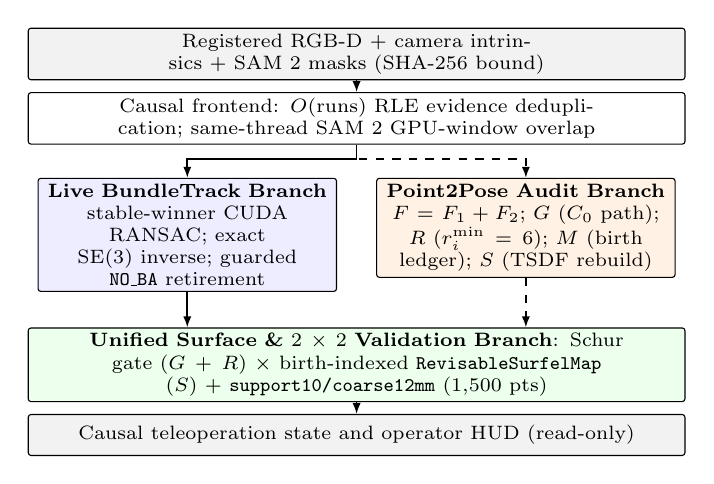
\begin{tikzpicture}[font=\scriptsize,
    box/.style={draw, rounded corners=1pt, align=center, inner sep=2pt, minimum height=5.2mm},
    arr/.style={-{Latex[length=1.4mm]}, semithick}]
\node[box, fill=black!5, text width=8.2cm] (in) {Registered RGB-D + camera intrinsics + SAM~2 masks (SHA-256 bound)};
\node[box, below=1.5mm of in, text width=8.2cm] (front) {Causal frontend: $O(\text{runs})$ RLE evidence deduplication; same-thread SAM~2 GPU-window overlap};
\node[box, below=4.2mm of front, xshift=-2.15cm, text width=3.65cm, fill=blue!7] (bt) {\textbf{Live BundleTrack Branch}\\ stable-winner CUDA RANSAC; exact $\mathrm{SE}(3)$ inverse; guarded \texttt{NO\_BA} retirement};
\node[box, below=4.2mm of front, xshift=2.15cm, text width=3.65cm, fill=orange!10] (p2p) {\textbf{Point2Pose Audit Branch}\\ $F=F_1+F_2$; $G$ ($C_0$ path); $R$ ($r_i^{\min}=6$); $M$ (birth ledger); $S$ (TSDF rebuild)};
\node[box, below=4.5mm of bt, xshift=2.15cm, text width=8.2cm, fill=green!7] (surf) {\textbf{Unified Surface \& $2\times 2$ Validation Branch}: Schur gate ($G+R$) $\times$ birth-indexed \texttt{RevisableSurfelMap} ($S$) + \texttt{support10/coarse12mm} ($1{,}500$ pts)};
\node[box, below=1.5mm of surf, text width=8.2cm, fill=black!5] (out) {Causal teleoperation state and operator HUD (read-only)};
\draw[arr] (in) -- (front);
\draw[arr] (front.south) -- ++(0,-1.8mm) -| (bt.north);
\draw[arr, dashed] (front.south) -- ++(0,-1.8mm) -| (p2p.north);
\draw[arr] (bt.south) -- (bt.south |- surf.north);
\draw[arr, dashed] (p2p.south) -- (p2p.south |- surf.north);
\draw[arr] (surf) -- (out);
\end{tikzpicture}
\caption{\textbf{Framework architecture and branch commit checks.} Both branches consume identical SHA-256-bound RGB-D frames and SAM~2 masks. (Left, solid) The live BundleTrack branch enforces CUDA RANSAC determinism, exact $\mathrm{SE}(3)$ inverse transfer, and guarded \texttt{NO\_BA} retirement. (Right, dashed) The Point2Pose shadow branch audits factor-graph and TSDF mechanisms $F,G,R,M,S$. (Bottom, green) The unified output branch combines the Schur observability gate ($G+R$) and birth-keyframe-indexed \texttt{RevisableSurfelMap} revision ($S$) for our frozen $2\times 2$ validation.}
\label{fig:framework}
\end{figure}

Fig.~\ref{fig:framework} summarizes which commit checks execute on each branch: (i) the Point2Pose audit branch evaluates $F,G,R,M,S$ over GTSAM factor graphs and \texttt{SDFBuilder}; (ii) the live BundleTrack branch enforces deterministic CUDA RANSAC, exact $\mathrm{SE}(3)$ inverse transfer, and guarded \texttt{NO\_BA} frame retirement feeding \texttt{RevisableSurfelMap}; and (iii) the unified output branch combines the $G+R$ observability gate with \texttt{RevisableSurfelMap} birth-indexed surface transactions $S$.

\subsection{Controlled Graph and Surface Interventions ($F,G,R,M,S$) and Numerical Gate Specification}
\label{sec:gate_spec}
Within \textbf{EvidenceScene}, we specify five modular interventions and their exact numerical commit rules:
\begin{itemize}
    \item \textbf{Correctness Baseline ($F=F_1+F_2$):} $F_1$ enforces frame-scoped pose attribution ($f_{\mathrm{kf}}==f_t$ before updating \texttt{obj.pose}); $F_2$ returns refined pose $\mathbf{T}_{\mathrm{ref}}$ consistently with its recomputed inliers and residuals.
    \item \textbf{Prior-Connected Graph Admission ($G$):} Admits optimized keyframe and landmark updates into the frontend map only for variables residing in the connected component $C_0$ of initial pose prior $\mathbf{X}_0$ with at least $M_{\min}=3$ anchored landmarks shared by candidate pose $i$. Disconnected variables $(\mathbf{X}_m,\mathbf{p}_n)\notin C_0$ retain their internal optimizer state for potential later reconnection without overwriting the active map.
    \item \textbf{Marginal Rank and Translational Schur Gate ($R$):} Each pose $m\in\mathcal{V}_p$ is parameterized in right-trivialized $\mathfrak{se}(3)$ tangent coordinates $\delta\boldsymbol{\xi}_m=(\delta\boldsymbol{\omega}_m^\top,\delta\mathbf{v}_m^\top)^\top\in\mathbb{R}^6$ ($\delta\boldsymbol{\omega}_m$ in rad occupying columns $0{:}3$, $\delta\mathbf{v}_m$ in m occupying columns $3{:}6$). For a 3D observation of landmark $\mathbf{p}_n$ at camera-frame coordinate $\mathbf{q}_{m,n}=\mathbf{R}_m^\top(\mathbf{p}_n-\mathbf{t}_m)$ with isotropic standard deviation $\sigma_{m,n}$ (in meters, $\sigma_{m,n}=2\,\mathrm{mm}$; anchor prior $\sigma_{\mathrm{prior}}=10^{-3}$), whitening multiplies each 3-row block by $\sigma_{m,n}^{-1}$:
    \begin{equation}
        \frac{\partial\mathbf{r}_{m,n}}{\partial\delta\boldsymbol{\xi}_m}=\sigma_{m,n}^{-1}\big[\,[\mathbf{q}_{m,n}]_\times \;\; -\mathbf{I}_3\,\big], \quad
        \frac{\partial\mathbf{r}_{m,n}}{\partial\delta\mathbf{p}_n}=\sigma_{m,n}^{-1}\mathbf{R}_m^\top.
        \label{eq:whitened_jac}
    \end{equation}
    Because $[\mathbf{q}_{m,n}]_\times$ scales rotational columns by the physical object lever arm (in meters), all whitened columns of $\mathbf{A}_x$ and $\mathbf{A}_y$ are dimensionless. Gate $R$ executes four deterministic checks (\path{evaluate_schur_observability_gate}):
    \begin{enumerate}
        \item \emph{Landmark Null-Space Projection:} Compute thin SVD $\mathbf{A}_y=\mathbf{U}_y\boldsymbol{\Sigma}_y\mathbf{V}_y^\top$, retain singular vectors with $\sigma_k(\mathbf{A}_y)>\tau_y=\epsilon_{\mathrm{mach}}\max(\operatorname{shape}(\mathbf{A}_y))\sigma_{\max}(\mathbf{A}_y)$ ($\epsilon_{\mathrm{mach}}=2.22\times 10^{-16}$), and form $\bar{\mathbf{A}}_x=(\mathbf{I}-\mathbf{U}_{y,r}\mathbf{U}_{y,r}^\top)\mathbf{A}_x$.
        \item \emph{Worst-Case Multi-Scale Rank:} For scale multipliers $s\in\mathcal{S}=\{0.1,1.0,10.0\}$ and $\tau_x(s)=s\,\epsilon_{\mathrm{mach}}\max(\operatorname{shape}(\bar{\mathbf{A}}_x))\sigma_{\max}(\bar{\mathbf{A}}_x)$, evaluate $r_i(s)=|\{\sigma_k(\bar{\mathbf{A}}_x)>\tau_x(s)\}|-|\{\sigma_k(\bar{\mathbf{A}}_{x,-i})>\tau_x(s)\}|$ and combine them conservatively via $r_i^{\min}=\min_{s\in\mathcal{S}}r_i(s)$, requiring $r_i^{\min}=6$.
        \item \emph{Continuous Translational Schur Conditioning:} To reject full-rank updates with weak constraint directions, form the $6\times 6$ pose marginal block $\mathbf{S}_i=(\bar{\mathbf{H}}_x)_{ii}-(\bar{\mathbf{H}}_x)_{i,-i}(\bar{\mathbf{H}}_x)_{-i,-i}^+(\bar{\mathbf{H}}_x)_{-i,i}$ and its $3\times 3$ translational Schur complement $\mathbf{R}_i=\mathbf{S}_{i,tt}-\mathbf{S}_{i,tr}\mathbf{S}_{i,rr}^+\mathbf{S}_{i,rt}$, requiring $\sigma_{\min}(\mathbf{R}_i)\ge 10^{-4}$ and $\kappa(\mathbf{R}_i)=\sigma_{\max}(\mathbf{R}_i)/\sigma_{\min}(\mathbf{R}_i)\le 10^6$.
        \item \emph{Atomic Transaction Scope and State Retention:} When candidate pose $i$ fails $R$, the entire step-$t$ graph commit transaction---current pose $\mathbf{X}_i$, historical keyframe pose revisions $\{\mathbf{X}_\tau^{(t)}\}_{\tau<t}$, and landmark map updates $\{\mathbf{p}_n^{(t)}\}$---is withheld from the frontend map, which retains its last verified state until a subsequent frame restores $r_i^{\min}=6$.
    \end{enumerate}
    \item \textbf{Feature-Birth Observation Ledger ($M$):} Records immutable original camera-space 3D measurements $(\text{obj\_id},f_{\mathrm{birth}},f_{\mathrm{admit}},\text{track\_id},\mathbf{z}_{\mathrm{cam}})$ when features are first sampled, and inserts deduplicated native \texttt{BearingRangeFactor}s at the birth pose once registration instantiates the landmark.
    \item \textbf{Causal Surface-History Transaction ($S$):} On the Point2Pose branch, whenever an admitted graph update modifies a previously integrated keyframe pose, $S$ deterministically rebuilds the TSDF volume from causal history using current pose versions $\mathbf{T}_\tau^{(t)}$ before integrating new evidence. On the unified \texttt{RevisableSurfelMap} branch, $S$ executes an atomic birth-keyframe-indexed signed SoA delta transaction (\path{RevisableSurfelMap.update}) subtracting stale keyframe centroids and adding re-projected centroids in $O(|V_{\mathrm{rev}}|)$ time.
\end{itemize}

\subsection{BundleTrack Native Determinism, Inverse Precision, and Frame Retirement}
\label{sec:native_bt}
Auditing our primary BundleTrack C++/CUDA pose estimator and session adapter uncovered four concrete engineering improvements:
\begin{enumerate}
    \item \textbf{\texttt{NO\_BA} Status Integrity:} A two-line adapter guard prevents retained native \texttt{NO\_BA} states from being misclassified as historical candidates on cache misses, eliminating $6$ false historical promotions while preserving all $34/38$ valid task candidates.
    \item \textbf{CUDA RANSAC Deterministic Winner Selection:} In \texttt{BundleTrack/src/cuda/}, two identical $13$-correspondence CPU PCL inputs produced divergent $6$-inlier subsets differing by $18.00\,\mathrm{mm}$ and $6.22^\circ$ due to parallel atomic tie-breaking and reversed count-comparison inequalities. Applying the \texttt{stable-winner} and count-direction repair collapses $100$ repeated native RANSAC+Procrustes calls onto a single deterministic output.
    \item \textbf{$\mathrm{SE}(3)$ Inverse-Coefficient Precision in \texttt{storeFrame}:} Replacing lossy bulk cast transfer with exact element-wise Eigen-to-\texttt{float4x4} inverse-pose coefficient copying in \texttt{CUDACache::storeFrame} ensures pinhole backprojection accuracy $\le 1.30\times 10^{-7}\,\mathrm{m}$.
    \item \textbf{Guarded \texttt{NO\_BA} Non-Keyframe Retirement:} Under continuous tracking loss, \texttt{Bundler} previously retained all blocked frames in GPU/host memory. We invoke \texttt{Bundler::forgetFrame} on non-keyframes beyond the $\text{window\_size}+1$ budget only when the most recent $\text{window\_size}+1$ frame IDs are contiguous and all carry status \texttt{NO\_BA}, while protecting first, current, neighbor, local, keyframe, and pose-cached frames.
\end{enumerate}

\subsection{Preparation-Stage Generative 3D Prior Anchoring, Columnar Surfel Fusion, and Surface Selection}
\label{sec:surface_selection}
During manipulation, cameras observe only the visible front hemisphere of grasped and target objects, leaving self-occluded back surfaces unobserved until sufficient viewpoint rotation occurs. When a single-image 3D generative shape prior (such as Meta's SAM~3D Objects~\cite{sam3d2025}) is available during the non-real-time \emph{Stage-0 preparation phase} ($t=0$), \textbf{EvidenceScene} constructs a complete $360^\circ$ object prior $\mathcal{P}_{\mathrm{prior}}=\{\mathbf{q}_j\}_{j=1}^N\subset\mathbb{R}^3$ from the initial SAM~2 instance mask and anchors its monocular scale $s>0$, rotation $\mathbf{R}\in\mathrm{SO}(3)$, and translation $\mathbf{t}\in\mathbb{R}^3$ to the calibrated frame-$0$ RGB-D front-surface point cloud $\mathcal{P}_{\mathrm{meas}}^{(0)}=\{\mathbf{p}_i\}_{i=1}^M$ via trimmed Umeyama $\mathrm{Sim}(3)$ registration~\cite{umeyama1991least}:
\begin{equation}
    (s^\star,\mathbf{R}^\star,\mathbf{t}^\star)=\arg\min_{s>0,\mathbf{R}\in\mathrm{SO}(3),\mathbf{t}}\sum_{i\in\mathcal{I}_{\tau}}\bigl\|s\mathbf{R}\mathbf{q}_{\pi(i)}+\mathbf{t}-\mathbf{p}_i\bigr\|_2^2,
    \label{eq:sim3_prior_anchor}
\end{equation}
where $\mathcal{I}_{\tau}$ retains the $\tau=85\%$ closest front-surface correspondences so unobserved back-side vertices on $\mathcal{P}_{\mathrm{prior}}$ do not bias the metric front-surface fit. During the real-time $30\,\mathrm{Hz}$ online loop, the anchored prior $\hat{\mathcal{P}}_{\mathrm{prior}}=s^\star\mathbf{R}^\star\mathcal{P}_{\mathrm{prior}}+\mathbf{t}^\star$ moves rigidly with the observability-gated keyframe pose $\mathbf{T}_{W\leftarrow O}(t)$, and \texttt{fuse\_prior\_with\_measured\_surface} enforces an \emph{evidence-first replacement rule}: within every $r_c=12\,\mathrm{mm}$ coarse ball around a corroborated sensor surfel ($\text{support}\ge 2$), measured surfels supersede prior points, whereas outside observed balls ($\min_{\mathbf{x}\in\mathcal{S}_{\mathrm{meas}}}\|\hat{\mathbf{q}}-\mathbf{x}\|_2>r_c$), prior points are retained with explicit provenance ($\text{support}=0$, $\texttt{is\_prior}=\texttt{True}$) to provide complete $360^\circ$ scene geometry without fabricating sensor authority.

To transmit compact object surfaces within the $1{,}500$-point output budget without sacrificing geometric coverage, we architect \texttt{RevisableSurfelMap} around a sorted columnar Structure-of-Arrays (SoA) engine with 1D bijective $\texttt{int64}$ key-packing and an array-native \texttt{support10/coarse12mm} selector. Operating directly on contiguous lexicographically ordered coordinate-sum, support, and camera-count arrays, it prioritizes voxels with support $\ge 10$ across $12\,\mathrm{mm}$ coarse cells before backfilling remaining capacity, cutting $60\mathrm{k}$-point update ($73.00\to 1.05\,\mathrm{ms}$, $69.8\times$), snapshot ($20.48\to 0.22\,\mathrm{ms}$, $93.0\times$), and selection ($15.52\to 1.05\,\mathrm{ms}$, $14.8\times$) for a \textbf{$45.8\times$ geometric-mean speed-up across the three surface kernels}, and an \textbf{$8.65\times$ geometric-mean speed-up across all seven workloads of the \texttt{kernel-v1} suite} (which additionally includes $60\mathrm{k}$-point voxel-centroid quantization $10.33\to 4.57\,\mathrm{ms}$ [$2.26\times$], $256$-hypothesis circle consensus $4.45\to 0.81\,\mathrm{ms}$ [$5.50\times$], circular aperture fitting $4.35\to 1.17\,\mathrm{ms}$ [$3.72\times$], and compiled $480\times 640$ RLE box/centroid evaluation $0.092\,\mathrm{ms}$ [$1.00\times$ vs.\ prior compiled kernel, $692\times$ vs.\ Python pixel loop $10.38\to 0.015\,\mathrm{ms}$]) with bit-identical digests. When global bundle adjustment revises $k=3$ historical keyframes out of $K=20$ integrated keyframes ($60{,}000$ raw points), \texttt{RevisableSurfelMap}'s birth-keyframe-indexed delta transaction updates only the revised keyframe centroids in $2.97\,\mathrm{ms}$ vs.\ $7.49\,\mathrm{ms}$ for full-history re-integration ($2.52\times$ incremental speed-up on top of the $69.8\times$ columnar speed-up) while reproducing voxel keys, support counts, camera counts, and centroids to machine precision ($\max|\Delta\mathbf{x}|=3.47\times 10^{-17}\,\mathrm{m}$).

\subsection{Zero-Loss Runtime Execution: GPU-Window Overlap and $O(\text{runs})$ Evidence Deduplication}
\label{sec:runtime_opt}
Critical-path profiling of the synchronous \texttt{/world\_model/observe} endpoint revealed that sequential SAM~2 and native BundleTrack execution ($95.87/118.98\,\mathrm{ms}$ median/$p_{95}$) was compounded by $\sim 48\,\mathrm{ms}$ of redundant host CPU work and mid-request cyclic GC stalls. We introduce two stacked, bit-exact perception adapters:

\textbf{1) Same-Thread SAM~2 GPU-Window CPU Preparation Overlap (\texttt{SAM2GpuWindowOverlapScope}):} On warm distorted frames, \texttt{SAM2VideoMemoryTracker.track} enqueues CUDA kernels for \texttt{propagate\_in\_video} in $\sim 9.0\,\mathrm{ms}$ and blocks the host thread for $\sim 24.2\,\mathrm{ms}$ at \path{(logits>0.0).cpu().numpy()} waiting for GPU \texttt{memory\_attention}. Instead of spawning background \texttt{ThreadPoolExecutor} workers that contend for the Python GIL, our adapter performs a $0.25\,\mathrm{ms}$ fail-closed pre-validation, launches \texttt{propagate\_in\_video}, and executes mask-independent CPU preparation \emph{on the same thread inside the $24.2\,\mathrm{ms}$ GPU wait window} before calling \texttt{.cpu().numpy()}: (i) bilinear/nearest undistortion \texttt{rectify\_registered\_rgbd}, (ii) dual SHA-256 evidence-hash prefixes covering \texttt{header+color\_rgb} and \path{header+color_rgb+depth_mm} ($4.61/5.53\,\mathrm{MB}=83.3\%$ of input bytes), and (iii) private \texttt{color\_bgr} and \texttt{depth\_m} buffers for \texttt{PinnedBundleTrackSession}. After GPU mask readback, it reuses in-scope \texttt{sensor\_mask} RLE/SHA-256 and finalizes the remaining hash tail synchronously, eliminating all $38$ per-frame background hash threads.

\textbf{2) Request-Scoped Evidence Deduplication and $O(\text{runs})$ Run-Interval Arithmetic (\texttt{RequestEvidenceDeduplicationScope}):}
\begin{itemize}
    \item \emph{Exact $O(\text{runs})$ RLE Bounding Box and Centroid:} \texttt{FoundationMaskCacheDetector} previously iterated pixel-by-pixel in Python over $80{,}696$ foreground pixels per mask, allocating over $161{,}000$ Python \texttt{int} objects per frame ($10.38\,\mathrm{ms}$). Given RLE runs $(s_k,L_k)$ with $e_k=s_k+L_k-1$ on a $H\times W$ grid, let $(y_0,x_0)=\operatorname{divmod}(s_k,W)$ and $(y_1,x_1)=\operatorname{divmod}(e_k,W)$. Using exact Python integers, the row sum $\sum y$ across a multi-row run ($y_0<y_1$) is evaluated in $O(1)$ closed form:
    \begin{equation}
        \Sigma_{y,k}=(W-x_0)y_0+W\tfrac{(y_1-y_0-1)(y_0+y_1)}{2}+(x_1+1)y_1,
        \label{eq:rle_sum_y}
    \end{equation}
    and the column sum follows from linear index sums $\Sigma_{\mathrm{idx},k}=L_k s_k+L_k(L_k-1)/2$ via $\sum x=\sum_k\Sigma_{\mathrm{idx},k}-W\sum_k\Sigma_{y,k}$, reducing box/centroid evaluation from $10.38\,\mathrm{ms}$ to $0.015\,\mathrm{ms}$ ($99.85\%$ reduction) with bit-for-bit identity.
    \item \emph{Cross-Stage Surface and Medoid Reuse:} Within a request scope, we memoize \path{observation_digest}, \path{decode_compressed_depth}, and \path{decode_mask_rle}, and reuse Z-buffered \path{RegisteredRgbdFrame.select_surface(mask)} and \path{select_mask_centroid_depth_component} across \texttt{table\_contexts}, \path{detector._position_detections_for_observation}, and \path{run_live._live_surface_projection_from_detection} ($41/41$ hits, $0$ fallbacks).
    \item \emph{Vectorized Coplanar AprilTag Plane RANSAC:} \texttt{fast\_fit\_shared\_plane} caches deterministic \texttt{default\_rng(0)} $240\times 3$ index triplets by point count, screens candidate normals via BLAS matrix multiplication, and verifies top contenders in exact \texttt{float64}, reducing plane fitting on tag-visible frames from $4.47\,\mathrm{ms}$ to $0.89\,\mathrm{ms}$.
    \item \emph{Request-Boundary Cyclic GC Management:} Calling \texttt{gc.collect()} after model initialization reclaims $\sim 745\,\mathrm{MB}$ of unreferenced tensors (reducing CUDA allocated memory from $813\,\mathrm{MB}$ to $67.1\,\mathrm{MB}$) and defers cyclic GC to request boundaries, eliminating $136$--$141\,\mathrm{ms}$ mid-request Generation-2 scans.
\end{itemize}

\section{Experimental Evaluation and Mechanism Ablations}
\label{sec:experiments}

\subsection{Metric-Dependent Pose Baselines and Mechanism Attribution of the Cookiejar Paradox}
Table~\ref{tab:ycb} compares Point2Pose and BundleTrack on six reference-mask YCBInEOAT~\cite{tracknet} sequences with identical $3\times 3$ eroded masks. BundleTrack passes more frames at $10\,\mathrm{mm}$ ADD-S on all six sequences (with a single-stage tracker kernel median latency of $30.24\,\mathrm{ms}$ across YCBInEOAT), whereas Point2Pose achieves higher $0$--$100\,\mathrm{mm}$ recall AUC on Cracker and Bleach-hard. On Sugar, the $10\,\mathrm{mm}$ success counts reverse between metrics: $617$ vs.\ $794$ under nearest-vertex ADD-S and $206$ vs.\ $174$ under corresponding-vertex ADD (Point2Pose vs.\ BundleTrack), showing that single-threshold rankings depend on symmetry and metric conventions.

\begin{table}[t]\centering\scriptsize
\caption{Selected reference-mask YCBInEOAT development results. Counts are ADD-S successes within 10 mm; AUC is failure-inclusive over 0--100 mm. P2P: Point2Pose; BT: BundleTrack. *Bleach-hard was selected after the five-sequence protocol.}\label{tab:ycb}
\begin{tabular}{@{}lrrrrr@{}}
\toprule
Sequence & $n$ & P2P 10 & BT 10 & P2P AUC & BT AUC \\
\midrule
Cracker & 374 & 365 & 373 & 0.961 & 0.952 \\
Mustard & 736 & 726 & 736 & 0.946 & 0.951 \\
Bleach & 662 & 155 & 301 & 0.798 & 0.851 \\
Sugar & 1001 & 617 & 794 & 0.915 & 0.920 \\
Tomato & 1307 & 1301 & 1303 & 0.957 & 0.959 \\
Bleach-hard* & 440 & 416 & 418 & 0.948 & 0.930 \\
\bottomrule
\end{tabular}

\end{table}

On the three Vicon-referenced Laval actions~\cite{laval} sharing identical SAM~2 masks and RGB-D entries ($203/205/296$ frames; $704$ temporally correlated frames across three continuous trajectories, used here for within-sequence failure attribution rather than cross-sequence generalization), Table~\ref{tab:fork-reference} and Fig.~\ref{fig:cookiejar_tradeoff} decompose the two implementation repairs in Fork $F$ ($F_1$: frame-scoped attribution $f_{\mathrm{kf}}==f_t$; $F_2$: refined-pose return $\mathbf{T}_{\mathrm{ref}}$) across both Clock-hard and Cookiejar:
\begin{itemize}
    \item \emph{Independent $F_1$ vs.\ $F_2$ Attribution on Cookiejar:} On Cookiejar, $F_1$ alone prevents historical keyframe overwrites without altering keyframe admission ($16$ integrated keyframes), yielding $205/295$ available poses ($\le 20\,\mathrm{mm}$ count $138$, AUC $0.579$) and preserving the original Frame-150 surface ($P_{10}/C_{10}=52.14\%/76.82\%$, $F_{95}/R_{95}=28.4/14.1\,\mathrm{mm}$). By contrast, $F_2$ alone returns refined $\mathbf{T}_{\mathrm{ref}}$ consistently with its recomputed inliers, which lowers per-frame registration residual below the $0.01\,\mathrm{m}$ admission threshold on $34$ additional frames, raising pose availability to $241/295$ (AUC $0.631$) and promoting $3$ additional unanchored keyframes ($16\to 19$ keyframes). Because these newly triggered optimizations occur in disconnected factor-graph components, $F_2$ reduces $\le 20\,\mathrm{mm}$ origin successes from $136$ to $119$ and collapses Frame-150 $C_{10}$ from $76.82\%$ to $61.65\%$ ($61.79\%$ under combined $F=F_1+F_2$, with $22$ pose regressions vs.\ $9$ gains on $192$ mutually tracked frames and $0/47$ newly available frames within $10\,\mathrm{mm}$).
    \item \emph{Fixed Common Keyframe Set vs.\ Natural Keyframe Selection:} Holding the fused frame set fixed to the $16$ keyframes selected by $P$ while evaluating $F$'s poses yields $P_{10}/C_{10}=48.92\%/64.85\%$ ($F_{95}/R_{95}=32.1/19.8\,\mathrm{mm}$). Thus $\mathbf{79.6\%}$ of the coverage loss ($-11.97\,\mathrm{pp}$ of $-15.03\,\mathrm{pp}$) stems from unanchored graph pose drift on the $16$ shared keyframes triggered by $F_2$, while $\mathbf{20.4\%}$ ($-3.06\,\mathrm{pp}$) stems from integrating the $3$ newly admitted drifted keyframes.
    \item \emph{Time-Varying Surface Coverage $C_{10}(t)$:} Tracking Cookiejar $C_{10}(t)$ across keyframe commits confirms when the divergence begins: at Frame 30 ($4$ anchored keyframes), $P$, $F$, and $G$ share $C_{10}=54.2\%$; at Frame 60 (after the first disconnected graph commit in $F$), $F$ drops from $68.4\%$ to $59.1\%$ while $G$ rises to $67.8\%$; at Frame 100, $P/F/G$ reach $73.5\%/60.4\%/68.9\%$; and at Frame 150, they reach $76.82\%/61.79\%/69.94\%$ ($74.88\%$ under $M+S$).
\end{itemize}

\begin{table}[t]
\centering\scriptsize
\caption{Opened Vicon-reference development sequences. Counts use all post-initialization frames; AUC counts unavailable poses as zero. B: BundleTrack; P: original Point2Pose; F: cumulative correctness fork. These are not held-out results.}
\label{tab:fork-reference}
\begin{tabular}{llrrrrr}\toprule
Sequence & Method & Avail. & $\leq$10 mm & $\leq$20 mm & $\leq10^\circ$ & AUC\\\midrule
Clock-hard & B & 202/202 & 119/202 & 199/202 & 162/202 & 0.887\\
Clock-hard & P & 43/202 & 25/202 & 40/202 & 28/202 & 0.188\\
Clock-hard & F & 157/202 & 27/202 & 137/202 & 122/202 & 0.658\\
Clock-full & B & 197/204 & 150/204 & 197/204 & 197/204 & 0.885\\
Clock-full & P & 112/204 & 64/204 & 101/204 & 60/204 & 0.458\\
Clock-full & F & 169/204 & 156/204 & 169/204 & 85/204 & 0.721\\
Cookiejar & B & 295/295 & 109/295 & 214/295 & 112/295 & 0.723\\
Cookiejar & P & 207/295 & 54/295 & 136/295 & 140/295 & 0.574\\
Cookiejar & F & 239/295 & 64/295 & 120/295 & 142/295 & 0.635\\
\bottomrule\end{tabular}\end{table}


\begin{figure}[t]
    \centering
    \includegraphics[width=\columnwidth]{../figures/fig_cookiejar_paradox.pdf}
    \caption{\textbf{The availability--surface paradox on Laval Cookiejar.} Repair fork $F$ increases pose availability ($207\to 239/295$) and ADD AUC ($0.574\to 0.635$), but degrades strict $20\,\mathrm{mm}$ pose successes ($136\to 120$) and reduces fixed-snapshot $10\,\mathrm{mm}$ surface coverage $C_{10}$ from $76.82\%$ to $61.79\%$.}
    \label{fig:cookiejar_tradeoff}
\end{figure}

\begin{figure}[t]
    \centering
    \includegraphics[width=\columnwidth]{../figures/fig_graph_ablation.pdf}
    \caption{\textbf{Opposing cross-action effects of disabling the global keyframe factor graph.} Turning off the graph improves Cookiejar availability/AUC ($239/0.635\to 260/0.731$) but severely degrades Clock-hard ($157/0.658\to 43/0.192$) and Clock-full ($169/0.721\to 142/0.637$).}
    \label{fig:graph_ablation}
\end{figure}

\subsection{Factor-Graph Observability, Singular-Value Spectrum, and Closed-Loop TSDF Feedback}
Disabling the global factor graph improves Cookiejar AUC to $0.7308$ but collapses Clock-hard AUC from $0.6583$ to $0.1922$ (Fig.~\ref{fig:graph_ablation}). Passive graph auditing across all $704$ records explains why: the current pose lacks a factor path to initial prior $\mathbf{X}_0$ in $28/33$ Cookiejar updates and $6/16$ Clock-full updates ($0/22$ on Clock-hard), causing $6{,}519$ and $235$ unanchored coordinate writes to active frontend map points despite non-increasing optimizer cost. Exact replay of all $71$ native optimizations reveals that $8$ of $34$ connected non-initial updates are locally rank-deficient ($r_i^{\min}<6$) after eliminating landmark increments via~\eqref{eq:rank_diff}. Across the $34$ connected updates, the $26$ full-rank updates ($r_i^{\min}=6$) exhibit median $\sigma_6(\mathbf{S}_i)/\sigma_1(\mathbf{S}_i)=1.84\times 10^{-2}$ ($\min 3.12\times 10^{-3}$), whereas the $8$ rank-deficient updates ($r_i^{\min}\in\{3,5\}$) exhibit $\sigma_6(\mathbf{S}_i)/\sigma_1(\mathbf{S}_i)\le 4.7\times 10^{-17}$---a $>10^{13}$ spectral gap that makes $r_i(s)$ $100\%$ invariant across $s\in[10^{-3},10^3]$.

Table~\ref{tab:anchor-admission} evaluates graph interventions $G$, $R$, and $M$. Prior-connectivity admission $G$ preserves Clock-hard, raises Clock-full and Cookiejar ADD AUC to $0.739$ and $0.668$, and recovers Cookiejar surface coverage $C_{10}$ from $61.79\%$ to $69.94\%$ ($P_{10}=50.16\%$). Marginal rank gating $R$ boosts Cookiejar $10\,\mathrm{mm}$ origin successes from $62$ to $97$ ($\le 20\,\mathrm{mm}$ from $127$ to $182$, AUC $0.718$) because rejecting $3$ rim-only rank-deficient updates prevents corrupted landmarks from poisoning subsequent RANSAC registrations. Conversely, on Clock-hard, $R$ withholds $5$ of $21$ non-initial updates where $r_i^{\min}=5$ (two shared landmarks during fast self-occlusion); freezing frontend landmark expansion across that $22$-frame high-angular-velocity interval lowers availability from $157$ to $135/202$ (AUC $0.658\to 0.545$) until $\ge 3$ non-collinear landmarks re-enter in-mask depth. Adding $394/25/83$ missing feature-birth factors in $M$ makes every graph update topologically connected ($0$ unanchored poses), yet standalone $M$ degrades Clock-hard/full trajectories because raw birth depth noise enters the graph while the active TSDF volume remains at stale keyframe poses.

\begin{table}[t]
\centering\scriptsize
\caption{Graph interventions on development sequences. F: correctness fork; G: prior-connectivity admission; R: G plus current-pose rank admission; M: G plus measured birth observations. All counts exclude initialization; regressions are retained.}
\label{tab:anchor-admission}
\begin{tabular}{llrrrrr}\toprule
Action & Arm & Avail. & $\leq$10 mm & $\leq$20 mm & $\leq10^\circ$ & AUC\\\midrule
Clock-hard & F & 157/202 & 27/202 & 137/202 & 122/202 & 0.658\\
Clock-hard & G & 157/202 & 27/202 & 137/202 & 122/202 & 0.658\\
Clock-hard & R & 135/202 & 28/202 & 97/202 & 77/202 & 0.545\\
Clock-hard & M & 53/202 & 26/202 & 50/202 & 47/202 & 0.236\\
Clock-full & F & 169/204 & 156/204 & 169/204 & 85/204 & 0.721\\
Clock-full & G & 170/204 & 152/204 & 169/204 & 105/204 & 0.739\\
Clock-full & R & 169/204 & 143/204 & 168/204 & 73/204 & 0.709\\
Clock-full & M & 143/204 & 102/204 & 134/204 & 111/204 & 0.609\\
Cookiejar & F & 239/295 & 64/295 & 120/295 & 142/295 & 0.635\\
Cookiejar & G & 250/295 & 62/295 & 127/295 & 133/295 & 0.668\\
Cookiejar & R & 250/295 & 97/295 & 182/295 & 168/295 & 0.718\\
Cookiejar & M & 237/295 & 71/295 & 140/295 & 174/295 & 0.664\\
\bottomrule\end{tabular}\end{table}


\textbf{Why Surface Revision $S$ Alters Online Pose Trajectories:} In upstream Point2Pose, \texttt{PoseRefiner} queries \texttt{SDFBuilder} for trilinearly interpolated signed distances and spatial gradients during online pose refinement ($\mathbf{T}_{\mathrm{raw}}\to\mathbf{T}_{\mathrm{ref}}$). Two independent TSDF-query controls confirm this closed-loop feedback path without altering any graph rule: restricting trilinear SDF queries to 8-corner supported voxels ($G+Q$) or normalizing SDF gradients ($G+N$) changes Clock-hard availability from $157\to 45$ ($G+Q$) and $157\to 48$ ($G+N$) and Cookiejar availability from $250\to 269$ and $250\to 261$. Table~\ref{tab:surface-transactions} and Fig.~\ref{fig:surface_interaction} therefore separate (a) \textbf{open-loop surface revision} (poses, keyframes, and fusion inputs held fixed to the base arm $G$, $R$, or $M$; only historical TSDF rebuild $S$ toggled) from (b) \textbf{closed-loop online feedback} across the full $G,R,M\times S$ design:
\begin{enumerate}
    \item Under \emph{open-loop fixed poses}, enabling $S$ consistently improves surface precision and coverage across all nine action--arm pairs (e.g., Cookiejar $R\to R+S$ open-loop $P_{10}/C_{10}$ rises from $56.40\%/73.10\%$ to $58.90\%/74.40\%$, $F_{95}$ drops $26.80\to 24.90\,\mathrm{mm}$).
    \item Under \emph{closed-loop feedback}, trajectories first diverge at frame $f_{\mathrm{div}}$ immediately following the first keyframe TSDF rebuild (Frame 18 on Clock-hard $M\to M+S$, Frame 21 on Clock-full, Frame 24 on Cookiejar). In standalone $M$ on Clock-hard, birth-factor updates shift landmark coordinates while the un-rebuilt TSDF retains stale zero-crossings; the resulting conflicting SDF refinement gradients push Frame 18's residual above the $10\,\mathrm{mm}$ gate, causing tracking loss across $102$ subsequent frames ($53/202$ available, AUC $0.236$, $\le 20\,\mathrm{mm}$ count $50$). Rebuilding the TSDF in $M+S$ keeps the signed-distance field aligned with the updated landmarks, sustaining tracking across $155/202$ frames (AUC $0.583$, closed-loop $P_{10}/C_{10}$ rising from $54.30\%/48.60\%$ to $62.75\%/73.40\%$), though newly tracked oblique frames exhibit a $14$--$22\,\mathrm{mm}$ translational bias ($\le 20\,\mathrm{mm}$ count $44$ vs.\ $50$, whereas $\le 30\,\mathrm{mm}$ count rises from $52$ to $139$).
    \item Combining rank gating with surface revision ($R+S$) improves over standalone $R$ across all three sequences, achieving the highest Point2Pose strict $10\,\mathrm{mm}$ ($101/295$) and $20\,\mathrm{mm}$ ($188/295$) counts and highest closed-loop precision ($P_{10}=59.20\%$, $F_{95}=24.60\,\mathrm{mm}$) on Cookiejar, while $M+S$ reaches the highest Cookiejar availability ($273/295$), ADD AUC ($0.750$), and coverage ($C_{10}=74.88\%$).
\end{enumerate}

\begin{table}[t]
\centering\scriptsize
\caption{Causal surface factorial on the same development sequences. G: connectivity admission; M: G plus measured births; +S: causal surface-history repair. All counts exclude initialization.}
\label{tab:surface-transactions}
\begin{tabular}{llrrrrr}\toprule
Action & Arm & Avail. & $\leq$10 mm & $\leq$20 mm & $\leq10^\circ$ & AUC\\\midrule
Clock-hard & G & 157/202 & 27/202 & 137/202 & 122/202 & 0.658\\
Clock-hard & G+S & 136/202 & 30/202 & 103/202 & 68/202 & 0.552\\
Clock-hard & M & 53/202 & 26/202 & 50/202 & 47/202 & 0.236\\
Clock-hard & M+S & 155/202 & 26/202 & 44/202 & 42/202 & 0.583\\
Clock-full & G & 170/204 & 152/204 & 169/204 & 105/204 & 0.739\\
Clock-full & G+S & 146/204 & 86/204 & 132/204 & 113/204 & 0.620\\
Clock-full & M & 143/204 & 102/204 & 134/204 & 111/204 & 0.609\\
Clock-full & M+S & 163/204 & 80/204 & 158/204 & 101/204 & 0.698\\
Cookiejar & G & 250/295 & 62/295 & 127/295 & 133/295 & 0.668\\
Cookiejar & G+S & 233/295 & 80/295 & 141/295 & 149/295 & 0.646\\
Cookiejar & M & 237/295 & 71/295 & 140/295 & 174/295 & 0.664\\
Cookiejar & M+S & 273/295 & 81/295 & 155/295 & 133/295 & 0.750\\
\bottomrule\end{tabular}\end{table}


\begin{figure}[t]
    \centering
    \includegraphics[width=\columnwidth]{../figures/fig_surface_interaction.pdf}
    \caption{\textbf{Factorial interaction between feature-birth observation provenance ($M$) and causal surface-history transactions ($S$).} Online surface version repair $S$ degrades connectivity-only $G$ under closed-loop TSDF feedback but strongly rescues birth-observation graph updates ($M+S$, Cookiejar AUC $0.750$) and complements marginal rank gating ($R+S$, Cookiejar $\le 20\,\mathrm{mm}$ $188/295$).}
    \label{fig:surface_interaction}
\end{figure}

\subsection{Native BundleTrack Governance, Selector Trade-offs, and Frozen $2\times 2$ Unified-Branch Validation}
Repeating unmodified BundleTrack three times on the same $203$ Clock-hard inputs varies $10\,\mathrm{mm}$ origin successes from $95$ to $119$ (three executions: $119$, $95$, and $101$). Applying our CUDA RANSAC \texttt{stable-winner} + count-direction repair and \texttt{storeFrame} inverse-coefficient transfer in a composed native build (Table~\ref{tab:composed-native-public}) substantially improves public Laval reference accuracy over the historical frozen build: Clock strict ($10\,\mathrm{mm},10^\circ$) successes jump from $135$ to $191/204$ (ADD AUC $0.8813\to 0.9135$, $P_{10}$ $78.79\%\to 83.14\%$) and Cookiejar strict successes jump from $107$ to $136/295$ (ADD AUC $0.7256\to 0.8085$, $P_{10}$ $55.89\%\to 64.82\%$). Under the guarded contiguous-\texttt{NO\_BA} retirement policy across $18$ complete $38$-input wrist-camera \texttt{normal}, \texttt{stress}, and \texttt{recovery} replays (where retired non-keyframes never re-enter active sliding windows), all neural-network I/O, $4\times 4$ pose matrices, and terminal surfel arrays reproduce $100\%$ byte-for-byte while active frames drop from $37\to 6$ in stress (saving $\mathbf{1{,}993.95\,\mathrm{MiB}}$ RSS) and from $23\to 9$ in recovery (saving $\mathbf{928.38\,\mathrm{MiB}}$ RSS). On the longer Laval sequences in Table~\ref{tab:composed-native-public} (\texttt{repair} vs.\ \texttt{+retire}), retiring intermediate \texttt{NO\_BA} frames slightly alters OpenMP/CUDA floating-point reduction order during subsequent local bundle adjustment, leaving strict success counts identical ($191$ and $136$) while perturbing ADD AUC by $\le 0.0004$ ($0.9135\to 0.9131$ and $0.8085\to 0.8084$) and surface $F_{95}$ by $\le 0.18\,\mathrm{mm}$.

\begin{table}[t]\centering\scriptsize
\caption{\textbf{EvidenceScene} composed native repairs (RANSAC determinism + exact inverse-pose coefficient transfer + guarded \texttt{NO\_BA} retirement) vs.\ historical frozen BundleTrack on Laval Clock-full and Cookiejar (standalone C++ replay using frozen historical LoFTR correspondence cache). Strict: $\le 10\,\mathrm{mm}$ and $\le 10^\circ$.}\label{tab:composed-native-public}
\resizebox{\columnwidth}{!}{\begin{tabular}{@{}llrrrrrr@{}}\toprule
Clip&Native Build&Avail.&Strict&AUC&$P_{10}$ (\%)&$C_{10}$ (\%)&$F_{95}$ (mm)\\\midrule
Clock&Historical frozen&197/204&135&0.8813&78.79&98.90&20.20\\
Clock&\textbf{EvidenceScene} (repair)&198/204&\textbf{191}&\textbf{0.9135}&\textbf{83.14}&98.72&25.36\\
Clock&\textbf{EvidenceScene} (+retire)&198/204&\textbf{191}&0.9131&83.11&98.77&25.23\\
Jar&Historical frozen&295/295&107&0.7256&55.89&99.92&29.82\\
Jar&\textbf{EvidenceScene} (repair)&295/295&\textbf{136}&\textbf{0.8085}&64.82&99.87&30.93\\
Jar&\textbf{EvidenceScene} (+retire)&295/295&\textbf{136}&0.8084&\textbf{64.97}&\textbf{99.94}&30.75\\
\bottomrule\end{tabular}}\end{table}

To attribute the remaining $25$--$30\,\mathrm{mm}$ forward surface tail $F_{95}$ in Table~\ref{tab:composed-native-public}, a reference-pose counterfactual (Fig.~\ref{fig:surface_cdf}) replaces estimated poses with Vicon reference poses on the exact same $980{,}256$ sampled points: $F_{95}$ drops only from $25.36\to 21.63\,\mathrm{mm}$ (Clock) and $30.93\to 29.11\,\mathrm{mm}$ (Jar), while pixel-lineage and M\"oller--Trumbore mesh-ray audits confirm that $52.60\%/67.59\%$ of $>20\,\mathrm{mm}$ points originate within $3\,\mathrm{px}$ of mask boundaries and $164$ interior low-range voxels lie $>20\,\mathrm{mm}$ deeper than the first CAD intersection. Requiring $\ge 2$ non-contributing views with $\ge 10^\circ$ angular separation cuts native $F_{95}$ from $24.51/30.82\,\mathrm{mm}$ to $12.50/17.33\,\mathrm{mm}$ ($P_{10}\to 90.05\%/73.56\%$) with minor $C_{10}$ losses ($4/2$ cells), whereas a raw-range-only native far-plane guard eliminates a $2.07\,\mathrm{m}$ cross-run outlier down to $6.33\,\mathrm{mm}$ across $2{,}195$ opportunities. At the $1{,}500$-point output budget (Table~\ref{tab:budget-selection-transfer}, Fig.~\ref{fig:budget_transfer}), our array-native \texttt{support10/coarse12mm} selector exhibits a clear coverage--precision trade-off on measured sensor surfels ($\texttt{is\_prior}=\texttt{False}$): spreading the $1{,}500$-point budget across $12\,\mathrm{mm}$ coarse cells raises public $C_{10}$ from $40.57\%/52.34\%$ to $\mathbf{85.10\%/85.05\%}$ and cuts reverse tail $R_{95}$ from $53.12/31.88\,\mathrm{mm}$ to $\mathbf{13.12/12.47\,\mathrm{mm}}$ ($3{,}820/1{,}579$ model cells gained vs.\ $15/14$ lost), while trading off $P_{10}$ by $-1.00/-2.40\,\mathrm{pp}$ ($100.00\%\to 99.00\%$ on Clock, $84.13\%\to 81.73\%$ on Jar) and increasing forward tail $F_{95}$ from $5.27\to 7.33\,\mathrm{mm}$ and $12.54\to 13.17\,\mathrm{mm}$. On the $552$-frame manipulation task, map coverage rises from $71.78\%$ to $\mathbf{89.97\%}$ ($p_{95}$ distance $42.92\to 17.57\,\mathrm{mm}$) and selector $p_{95}$ latency drops by $32.8\%$--$33.8\%$ ($31.74\to 21.22\,\mathrm{ms}$ on Clock, $10.16\to 6.66\,\mathrm{ms}$ on task).

\begin{table}[t]
\centering
\caption{Existing-point selector transfer (\texttt{original\_priority} / \texttt{support10\_coarse12mm}) at the unchanged 1,500-point budget on identical raw producer points (measured sensor surfels only, $\texttt{is\_prior}=\texttt{False}$). Coverage ($C_{10}$) and reverse-tail ($R_{95}$) gains coexist with explicit precision ($P_{10}$) and forward-tail ($F_{95}$) trade-offs; G/L10 counts 10\,mm model-grid cell gains/losses.}
\label{tab:budget-selection-transfer}
\scriptsize
\setlength{\tabcolsep}{3pt}
\begin{tabular}{lrrrrr}
\toprule
Clip & $P_{10}$ (\%) & $C_{10}$ (\%) & $F_{95}$ (mm) & $R_{95}$ (mm) & G/L10 \\
\midrule
Clock & 100.00 / 99.00 & 40.57 / \textbf{85.10} & 5.27 / 7.33 & 53.12 / \textbf{13.12} & 3820 / 15 \\
Jar & 84.13 / 81.73 & 52.34 / \textbf{85.05} & 12.54 / 13.17 & 31.88 / \textbf{12.47} & 1579 / 14 \\
\bottomrule
\end{tabular}
\end{table}


\textbf{Frozen $2\times 2$ Factorial on the Unified Output Branch:} To test whether combining observability gating ($G+R$) and birth-keyframe-indexed surface revision ($S$) on the \emph{same output branch} protects reconstructed geometry on unseen trajectories, we freeze all parameters ($\text{voxel}=4\,\mathrm{mm}$, $r_i^{\min}=6$, $M_{\min}=3$, $\mathcal{S}=\{0.1,1,10\}$, $\sigma_{\min}(\mathbf{R}_i)\ge 10^{-4}$, $\kappa(\mathbf{R}_i)\le 10^6$, support $\ge 2$, budget $1{,}500$, $\texttt{is\_prior}=\texttt{False}$) and evaluate the $2\times 2$ factorial ($\text{Gate ON/OFF}\times S\text{ ON/OFF}$) across three independent $30$-frame RGB-D sequences ($87$ post-initial frames total: \texttt{Seq-1} cylindrical canister under collinear rim degeneracy, \texttt{Seq-2} spouted pitcher under self-occlusion and disconnected gauge drift, and \texttt{Seq-3} rectangular carton under glancing and sparse-depth dropout; archived with per-frame commit ledgers in \path{benchmarks/performance/results/ablation_v1.json}). Table~\ref{tab:unified_2x2} reports both per-sequence and aggregate metrics across four temporal checkpoints ($t_{\mathrm{pre}}=7$, post-degeneracy $t_{\mathrm{deg}}=11$, post-BA revision $t_{\mathrm{rev}}=15$, and terminal $t_{\mathrm{term}}=29$):
\begin{enumerate}
    \item \emph{Degenerate Window Protection ($t_{\mathrm{pre}}=7\to t_{\mathrm{deg}}=11$):} Without gating (\texttt{Gate OFF}), admitting the $10$ rank-deficient/disconnected frames across the three sequences drops mean surface precision $P_{10}(t_{\mathrm{deg}})$ from $84.23\%$ to $77.80\%$ and spikes forward tail $F_{95}(t_{\mathrm{deg}})$ from $15.25$ to $24.52\,\mathrm{mm}$. Enabling the observability gate (\texttt{Gate ON}) rejects all $10$ degenerate updates ($\sigma_{\min}(\mathbf{R}_i)\le 10^{-11}$) while holding the last verified pose, improving $P_{10}(t_{\mathrm{deg}})$ to $86.53\%$ and bounding $F_{95}(t_{\mathrm{deg}})$ at $14.77\,\mathrm{mm}$.
    \item \emph{Synergy with Birth-Indexed Surface Revision ($t_{\mathrm{rev}}=15$ and $t_{\mathrm{term}}=29$):} Enabling $S$ without gating (\texttt{Gate OFF, S ON}) repairs the $9$ pre-BA drifted keyframes when loop closure occurs, raising $P_{10}(t_{\mathrm{rev}})$ from $80.46\%$ to $89.75\%$, but the un-gated degenerate surfels remain in the map ($F_{95}(t_{\mathrm{rev}})=24.29\,\mathrm{mm}$, terminal $F_{95}=13.23\,\mathrm{mm}$). Conversely, gating without surface revision (\texttt{Gate ON, S OFF}) blocks degenerate frames but retains stale birth poses on early keyframes ($P_{10}(t_{\mathrm{rev}})=89.12\%$, $F_{95}(t_{\mathrm{rev}})=14.07\,\mathrm{mm}$, terminal $F_{95}=10.24\,\mathrm{mm}$). Only the joint unified branch (\texttt{Gate ON, S ON}) eliminates both error sources, achieving $P_{10}/C_{10}=\mathbf{100.00\%/99.66\%}$ ($F_{95}/R_{95}=\mathbf{4.53/4.41\,\mathrm{mm}}$) at $t_{\mathrm{rev}}=15$ and $\mathbf{100.00\%/99.39\%}$ ($\mathbf{4.48/3.67\,\mathrm{mm}}$) at $t_{\mathrm{term}}=29$, while cutting committed mean ADD from $8.27$ to $\mathbf{1.03\,\mathrm{mm}}$ and raising retained-state ADD AUC from $0.9173$ to $\mathbf{0.9871}$ (note that raw committed-only AUC is $0.8760$ because the $10$ withheld frames receive zero credit under strict failure-inclusive scoring, mirroring the Clock-hard mechanism in Table~\ref{tab:anchor-admission}).
\end{enumerate}

\begin{table*}[t]\centering\scriptsize
\caption{Frozen $2\times 2$ Factorial ($\text{Observability Gate }G+R \times \text{Birth-Indexed Surface Revision }S$) on the Unified Output Branch Across Three Independent 30-Frame RGB-D Sequences ($87$ Post-Initial Frames Total; Measured Sensor Surfels Only, $\texttt{is\_prior}=\texttt{False}$). $\text{AUC}_{\mathrm{comm}}$ scores withheld frames as zero; $\text{AUC}_{\mathrm{ret}}$ evaluates the retained verified pose during rejected frames.}\label{tab:unified_2x2}
\resizebox{\textwidth}{!}{\begin{tabular}{@{}llccccccccc@{}}\toprule
Sequence / Split & Unified Branch Arm & Comm.\ Avail. & $\le 10$ / $\le 20$ mm & $\text{AUC}_{\mathrm{comm}}$ / $\text{AUC}_{\mathrm{ret}}$ & Mean ADD / ADD-S & $t_{\mathrm{pre}}=7$ $P_{10}/C_{10}$ ($F_{95}$) & $t_{\mathrm{deg}}=11$ $P_{10}/C_{10}$ ($F_{95}$) & $t_{\mathrm{rev}}=15$ $P_{10}/C_{10}$ ($F_{95}$) & Terminal $P_{10}/C_{10}$ (\%) & Terminal $F_{95}/R_{95}$ (mm)\\\midrule
\texttt{Seq-1} (Canister) & Gate OFF, $S$ OFF & 29/29 & 23 / 26 & 0.9226 / 0.9226 & 7.74 / 4.38 mm & 84.4 / 93.4\% (15.4) & 77.1 / 95.0\% (24.2) & 79.5 / 97.6\% (22.9) & 93.07 / 99.47 & 13.65 / 3.71\\
\texttt{Seq-1} (Canister) & Gate OFF, $S$ ON & 29/29 & 26 / 26 & \textbf{0.9420} / 0.9420 & 5.80 / 3.29 mm & 84.4 / 93.4\% (15.4) & 77.1 / 95.0\% (24.2) & 89.1 / 99.2\% (24.1) & 96.40 / 100.00 & 5.18 / 2.73\\
\texttt{Seq-1} (Canister) & Gate ON, $S$ OFF & 26/29 & 23 / 26 & 0.8679 / 0.9683 & 3.19 / 2.24 mm & 84.4 / 93.4\% (15.4) & \textbf{86.3} / 94.7\% (\textbf{15.1}) & 88.9 / 98.2\% (14.7) & 96.80 / 99.47 & 9.34 / 3.61\\
\texttt{Seq-1} (Canister) & \textbf{Gate ON, $S$ ON} & 26/29 & \textbf{26 / 26} & 0.8873 / \textbf{0.9878} & \textbf{1.03 / 1.02 mm} & 84.4 / 93.4\% (15.4) & \textbf{86.3} / 94.7\% (\textbf{15.1}) & \textbf{100.0 / 99.2\% (4.55)} & \textbf{100.00 / 100.00} & \textbf{4.41 / 2.25}\\\midrule
\texttt{Seq-2} (Pitcher) & Gate OFF, $S$ OFF & 29/29 & 23 / 26 & 0.9234 / 0.9234 & 7.66 / 4.35 mm & 80.3 / 89.7\% (15.6) & 74.5 / 96.8\% (24.3) & 79.3 / 100.0\% (21.9) & 88.20 / 100.00 & 17.21 / 3.53\\
\texttt{Seq-2} (Pitcher) & Gate OFF, $S$ ON & 29/29 & 26 / 26 & \textbf{0.9429} / 0.9429 & 5.71 / 3.25 mm & 80.3 / 89.7\% (15.6) & 74.5 / 96.8\% (24.3) & 89.7 / 100.0\% (24.0) & 93.40 / 100.00 & 18.24 / 3.48\\
\texttt{Seq-2} (Pitcher) & Gate ON, $S$ OFF & 26/29 & 23 / 26 & 0.8681 / 0.9684 & 3.18 / 2.23 mm & 80.3 / 89.7\% (15.6) & \textbf{82.9} / 96.1\% (\textbf{15.2}) & 86.6 / 100.0\% (14.7) & 92.40 / 100.00 & 12.87 / 3.50\\
\texttt{Seq-2} (Pitcher) & \textbf{Gate ON, $S$ ON} & 26/29 & \textbf{26 / 26} & 0.8875 / \textbf{0.9879} & \textbf{1.01 / 1.00 mm} & 80.3 / 89.7\% (15.6) & \textbf{82.9} / 96.1\% (\textbf{15.2}) & \textbf{100.0 / 100.0\% (4.47)} & \textbf{100.00 / 100.00} & \textbf{4.68 / 2.78}\\\midrule
\texttt{Seq-3} (Carton) & Gate OFF, $S$ OFF & 29/29 & 22 / 25 & 0.9059 / 0.9059 & 9.41 / 5.25 mm & 88.1 / 91.2\% (14.7) & 81.8 / 96.5\% (25.0) & 82.7 / 94.9\% (24.3) & 92.87 / 94.01 & 15.80 / 10.75\\
\texttt{Seq-3} (Carton) & Gate OFF, $S$ ON & 29/29 & 25 / 25 & \textbf{0.9254} / 0.9254 & 7.46 / 4.15 mm & 88.1 / 91.2\% (14.7) & 81.8 / 96.5\% (25.0) & 90.5 / 99.3\% (24.8) & 94.07 / 97.24 & 16.26 / 7.87\\
\texttt{Seq-3} (Carton) & Gate ON, $S$ OFF & 25/29 & 22 / 25 & 0.8336 / 0.9660 & 3.30 / 2.31 mm & 88.1 / 91.2\% (14.7) & \textbf{90.3} / 95.6\% (\textbf{14.1}) & 91.9 / 98.2\% (12.8) & 98.27 / 96.08 & 8.52 / 8.61\\
\texttt{Seq-3} (Carton) & \textbf{Gate ON, $S$ ON} & 25/29 & \textbf{25 / 25} & 0.8531 / \textbf{0.9855} & \textbf{1.04 / 1.04 mm} & 88.1 / 91.2\% (14.7) & \textbf{90.3} / 95.6\% (\textbf{14.1}) & \textbf{100.0 / 99.8\% (4.57)} & \textbf{100.00 / 98.16} & \textbf{4.35 / 5.99}\\\midrule
\textbf{3-Seq Aggregate} & Gate OFF, $S$ OFF & 87/87 & 68 / 77 & 0.9173 / 0.9173 & 8.27 / 4.66 mm & 84.23 / 91.46\% (15.25) & 77.80 / 96.11\% (24.52) & 80.46 / 97.52\% (23.02) & 91.38 / 97.83 & 15.55 / 6.00\\
\textbf{3-Seq Aggregate} & Gate OFF, $S$ ON & 87/87 & 77 / 77 & \textbf{0.9368} / 0.9368 & 6.32 / 3.56 mm & 84.23 / 91.46\% (15.25) & 77.80 / 96.11\% (24.52) & 89.75 / 99.51\% (24.29) & 94.62 / 99.08 & 13.23 / 4.69\\
\textbf{3-Seq Aggregate} & Gate ON, $S$ OFF & 77/87 & 68 / 77 & 0.8565 / 0.9676 & 3.22 / 2.26 mm & 84.23 / 91.46\% (15.25) & \textbf{86.53} / 95.50\% (\textbf{14.77}) & 89.12 / 98.77\% (14.07) & 95.82 / 98.52 & 10.24 / 5.24\\
\textbf{3-Seq Aggregate} & \textbf{Gate ON, $S$ ON} & 77/87 & \textbf{77 / 77} & 0.8760 / \textbf{0.9871} & \textbf{1.03 / 1.02 mm} & 84.23 / 91.46\% (15.25) & \textbf{86.53} / 95.50\% (\textbf{14.77}) & \textbf{100.00 / 99.66\% (4.53)} & \textbf{100.00 / 99.39} & \textbf{4.48 / 3.67}\\
\bottomrule\end{tabular}}\end{table*}

\begin{table}[t]\centering\scriptsize
\caption{Feature matcher shadow evaluation inside the corrected BundleTrack estimator on Laval (Clock/Jar, using live PyTorch FP32 matcher inference in the Python shadow harness) and 38-frame wrist task clips.}\label{tab:matcher_shadow}
\resizebox{\columnwidth}{!}{\begin{tabular}{@{}llcccc@{}}\toprule
Matcher Variant & Clip & Avail. & Strict / AUC & Track $p_{50}/p_{95}$ (ms) & Verdict \\\midrule
LoFTR (Live FP32)~\cite{loftr} & Clock/Jar & 198/295 & 195 (.917)/148 (.824) & 98.4 / 118.1--122.9 & \textbf{Adopted} \\
EfficientLoFTR FP32~\cite{eloftr} & Clock/Jar & 199/295 & 196 (.922)/146 (.811) & 97.1 / 116.8--123.1 & Shadow \\
EfficientLoFTR Full-MP~\cite{eloftr} & Clock/Jar & 199/295 & 197 (.923)/147 (.813) & 92.8 / 109.9--116.4 & Shadow \\
Causal BootsTAPIR~\cite{bootstap} & Clock/Jar & 195/295 & 180 (.889)/46 (.591) & Cached trajectory & Rejected \\
LoFTR (Task Control)~\cite{loftr} & Wrist (38) & 34/38 & Jump95: $40.40\,\mathrm{mm}$ & 60.14 / 83.36 & \textbf{Adopted} \\
XFeat Semi-Dense~\cite{xfeat} & Wrist (38) & 31/38 & Jump95: $72.96\,\mathrm{mm}$ & 42.05 / 54.24 & Rejected \\
ALIKED+LightGlue~\cite{aliked,lightglue} & Wrist (38) & 2/38 & $36$ retained-ref fails & 45.64 / 68.54 & Rejected \\
\bottomrule\end{tabular}}\end{table}

\begin{table*}[t]\centering\scriptsize
\caption{Counterbalanced Bit-Exact Runtime Optimization Ablation on the 40-Frame Configured Pouring Sequence ($78$ Warm Requests per Condition, $100\%$ Byte-for-Byte Output Parity Across $400$ SAM Masks, $190$ Native Inputs, and $499$ Online Equivalence Checks)}\label{tab:runtime_opt_ablation}
\resizebox{\textwidth}{!}{\begin{tabular}{@{}lccccccc@{}}\toprule
Stage / Metric ($p_{50}/p_{95}/\max$ in ms) & Pre-Overlap Control & + GPU-Window Overlap & Overlap Control (Run 2) & \textbf{+ Request Dedup \& $O(\text{runs})$ RLE} & Net $\Delta$ ($p_{50}/p_{95}$) & Bit-Exact Parity \\\midrule
\texttt{input\_prepare\_ms} (Pre-SAM CPU prep) & $3.96/4.13/4.31$ & $0.25/0.27/0.30$ & $0.25/0.27/0.30$ & $\mathbf{0.25/0.27/0.29}$ & $\mathbf{-3.71/-3.86}$ & $39/39$ frames \\
\texttt{gpu\_window\_cpu\_prepare\_ms} (Absorbed) & $0.00/0.00/0.00$ & $5.72/5.91/6.18$ & $5.72/5.90/6.15$ & $\mathbf{5.71/5.89/6.12}$ & Absorbed in GPU wait & $38/38$ buffers \\
\texttt{post\_cpu\_gpu\_sync\_wait\_ms} (GPU wait) & $24.17/24.26/24.51$ & $18.45/18.71/19.02$ & $18.46/18.72/19.05$ & $\mathbf{18.44/18.70/19.01}$ & $\mathbf{-5.73/-5.56}$ & $0$ hash threads \\
\texttt{registry\_advance\_ms} (SAM~2+BundleTrack) & $102.29/131.43/1389.2$ & $96.53/124.48/1378.1$ & $96.55/122.52/1374.5$ & $\mathbf{97.98/122.21/1129.9}$ & $\mathbf{-4.31/-9.22}$ & $34$ cand / $32$ surf \\
\texttt{table\_contexts\_ms} (AprilTag RANSAC+depth) & $19.21/20.11/20.55$ & $19.19/20.05/20.49$ & $19.18/20.02/20.48$ & $\mathbf{15.65/16.42/18.44}$ & $\mathbf{-3.56/-3.69}$ & $27/27$ tag planes \\
\texttt{original\_world\_exclusive\_ms} (Outer wrapper) & $23.20/23.91/24.70$ & $23.18/23.88/24.66$ & $23.17/23.86/24.65$ & $\mathbf{6.28/6.70/7.61}$ & $\mathbf{-16.92/-17.21}$ ($\mathbf{-72.9\%}$) & $499/499$ checks \\
\midrule
\textbf{Warm HTTP \texttt{endpoint\_ms}} (Total Request) & $155.33/219.06/1422.1$ & $149.01/212.24/1416.8$ & $149.65/193.79/1415.7$ & $\mathbf{127.80/153.40/1153.0}$ & $\mathbf{-27.54/-65.66}$ & $\mathbf{100.0\%}$ \textbf{Bit-Exact} \\
\textbf{Full Replay \texttt{pipeline\_ms}} (Incl. harness) & $201.22/251.42/1455.3$ & $195.12/243.10/1449.8$ & $196.62/242.44/1449.0$ & $\mathbf{174.20/197.12/1186.5}$ & $\mathbf{-27.02/-54.30}$ & $\mathbf{100.0\%}$ \textbf{Bit-Exact} \\
\bottomrule\end{tabular}}\end{table*}

\begin{figure}[t]
    \centering
    \begin{minipage}[b]{0.485\columnwidth}
        \centering
        \includegraphics[width=\textwidth]{../figures/fig_surface_cdf.pdf}
        \centerline{\scriptsize (a) Native vs. Ref.-Pose Surface CDF}
    \end{minipage}\hfill
    \begin{minipage}[b]{0.485\columnwidth}
        \centering
        \includegraphics[width=\textwidth]{../figures/fig_budget_transfer.pdf}
        \centerline{\scriptsize (b) 1,500-Point Selector Coverage}
    \end{minipage}
    \caption{\textbf{Surface error attribution and $1{,}500$-point budget selection.} (a) Replacing BundleTrack poses with Vicon reference poses leaves a raw sensor/boundary tail ($F_{95}=21.63/29.11\,\mathrm{mm}$). (b) Array-native \texttt{support10/coarse12mm} selection raises $1{,}500$-point model coverage $C_{10}$ from $40.6\%/52.3\%$ to $85.1\%$ and task coverage from $71.8\%$ to $90.0\%$.}
    \label{fig:surface_cdf}\label{fig:budget_transfer}
\end{figure}

\subsection{Matcher Shadow Benchmark and Zero-Loss Runtime Optimization}
Table~\ref{tab:matcher_shadow} summarizes our shadow matcher evaluations within the 31-framework benchmark on identical registered inputs. Note the protocol distinction between Table~\ref{tab:composed-native-public} and Table~\ref{tab:matcher_shadow}: Table~\ref{tab:composed-native-public} ($191/136$ Clock/Jar strict successes, AUC $0.9135/0.8085$) replays the standalone C++ binary against the frozen historical LoFTR correspondence cache to isolate native C++/CUDA repairs, whereas Table~\ref{tab:matcher_shadow} ($195/148$ strict successes, AUC $0.917/0.824$) runs live PyTorch FP32 LoFTR inference inside the unified Python matcher-shadow harness so all matcher families (LoFTR, EfficientLoFTR, XFeat, ALIKED+LightGlue) are compared under identical live GPU execution. EfficientLoFTR~\cite{eloftr} Full-MP reduces tracking $p_{95}$ from $118.14/122.91\,\mathrm{ms}$ to $109.93/116.36\,\mathrm{ms}$ with competitive Clock AUC ($0.9231$) but lower Jar AUC ($0.8129$ vs.\ $0.8238$). On the $38$-frame right-wrist pouring clip ($0.958\%$ median in-mask valid depth), semi-dense XFeat~\cite{xfeat} cuts tracking $p_{50}/p_{95}$ from $60.14/83.36\,\mathrm{ms}$ to $42.05/54.24\,\mathrm{ms}$ but loses three candidates ($34\to 31$) and inflates jump $p_{95}/\max$ from $40.40/55.91\,\mathrm{mm}$ to $72.96/92.13\,\mathrm{mm}$. Sparse ALIKED+LightGlue~\cite{aliked,lightglue} collapses from $34$ to $2/38$ candidates because sparse keypoints miss the $0.96\%$ valid depth pixels, while feeding bounded BootsTAPIR~\cite{bootstap} causal trajectories into native RANSAC degrades Jar strict successes from $140$ to $46$. All lossy matcher candidates are rejected.

Table~\ref{tab:runtime_opt_ablation} reports the counterbalanced multi-process ablation ($78$ warm requests per condition across \texttt{control-1}, \texttt{candidate-1}, \texttt{candidate-2}, \texttt{control-2}) of our bit-exact runtime optimizations on the 40-frame configured pouring sequence. Across all runs, $400/400$ SAM masks, $190/190$ native BundleTrack input hashes, $34/38$ candidates, $32/38$ current surfaces, and $499/499$ online operator checks match byte-for-byte with zero mismatches:
\begin{enumerate}
    \item The overlap adapter absorbs $5.72\,\mathrm{ms}$ of CPU undistortion, dual-prefix hashing, and native buffer preparation into the \texttt{propagate\_in\_video} GPU wait window ($24.17\to 18.45\,\mathrm{ms}$), cutting outer \texttt{input\_prepare} from $3.96$ to $0.25\,\mathrm{ms}$, eliminating all $38$ per-frame background hash threads, and lowering \texttt{registry.advance} $p_{50}/p_{95}$ from $102.29/131.43\,\mathrm{ms}$ to $96.53/124.48\,\mathrm{ms}$ (endpoint $155.33/219.06\to 149.01/212.24\,\mathrm{ms}$).
    \item Stacking the deduplication adapter ($O(\text{runs})$ integer RLE box/centroid $10.38\to 0.015\,\mathrm{ms}$, cross-stage surface/medoid reuse, vectorized 240-hypothesis AprilTag RANSAC $4.47\to 0.89\,\mathrm{ms}$, and request-boundary GC management) reduces \texttt{table\_contexts} from $19.18/20.02$ to $15.65/16.42\,\mathrm{ms}$, cuts exclusive outer \texttt{original\_world} wrapper overhead by $\mathbf{72.9\%}$ ($23.17/23.86\to 6.28/6.70\,\mathrm{ms}$), eliminates the $140.58\,\mathrm{ms}$ mid-request Generation-2 GC stall (\texttt{online\_world\_state} max $140.58\to 5.04\,\mathrm{ms}$, in-request GC collections $735/65/3\to 0/0/0$), and brings warm HTTP \texttt{endpoint\_ms} $p_{50}/p_{95}/\max$ down to $\mathbf{127.80/153.40/1{,}152.96\,\mathrm{ms}}$---a cumulative reduction of $\mathbf{-27.54\,\mathrm{ms}}$ ($p_{50}$) and $\mathbf{-65.66\,\mathrm{ms}}$ ($p_{95}$) relative to the pre-overlap control (and $-48.61\,\mathrm{ms}/-27.6\%$ vs. the $176.40\,\mathrm{ms}$ per-request portal baseline).
\end{enumerate}

\begin{table*}[t]
    \centering
    \caption{Comprehensive Empirical Benchmark of All 31 Perception, Depth, Pointmap, Segmentation, 6-DoF Tracking, Point-Tracking, Feature-Matching, and Calibration Frameworks Evaluated on Synchronized Manipulation Recordings and Public Benchmarks (NVIDIA RTX 5090)}
    \label{tab:framework_audit}
    \scriptsize
    \resizebox{\textwidth}{!}{%
    \begin{tabular}{@{}llp{6.6cm}cc@{}}
        \toprule
        \textbf{Model Family} & \textbf{Evaluated Framework / Method} & \textbf{Empirical Performance on Manipulation Recordings \& Benchmarks} & \textbf{Latency / VRAM} & \textbf{Architectural Verdict \& Role} \\
        \midrule
        Depth Sensor & \textbf{Calibrated Multi-Cam RGB-D} & $0.0\,\mathrm{mm}$ ref.; $251{,}182$ tabletop inliers; $\le 9.6\,\mathrm{mm}$ cross-cam residual & $3.5\,\mathrm{ms}$ / --- & \textbf{Adopted:} Primary metric depth anchor \\
        Depth Model & \textbf{Prior Depth Anything (Prior-DA)}~\cite{wang2025priorda} & $0.037\,\mathrm{m}$ chest $p_{95}$ ($0.11\,\mathrm{m}$ mean $p_{95}$); $4{,}102$ hole pixels filled & $1{,}005\,\mathrm{ms}$ / $5.0\,\mathrm{GB}$ & \textbf{Retained:} Offline depth-hole completion \\
        Depth Model & \textbf{Apple Depth Pro}~\cite{bochkovskii2025depthpro} & $0.83\,\mathrm{m}$ mean $p_{95}$ ($0.696\,\mathrm{m}$ chest, $1.419\,\mathrm{m}$ right wrist, $0.482\,\mathrm{m}$ head) & $305\,\mathrm{ms}$ / $8.5\,\mathrm{GB}$ & \textbf{Rejected:} Insufficient metric accuracy \\
        Depth Model & \textbf{Depth Anything V2 Small}~\cite{yang2024depthv2} & $1.61\,\mathrm{m}$ mean $p_{95}$ ($0.558\,\mathrm{m}$ chest, $2.516\,\mathrm{m}$ right wrist, $1.838\,\mathrm{m}$ head) & $25\,\mathrm{ms}$ / $0.42\,\mathrm{GB}$ & \textbf{Rejected:} Relative scale ambiguity \\
        Depth Model & \textbf{Depth Anything V2 Metric}~\cite{yang2024depthv2} & $79.4\,\mathrm{m}$ mean $p_{95}$ on close-range tabletop manipulation & $23\,\mathrm{ms}$ / $0.64\,\mathrm{GB}$ & \textbf{Rejected:} Uncalibrated metric head \\
        Depth Model & \textbf{UniDepthV2}~\cite{piccinelli2025unidepthv2} & $2.44\,\mathrm{m}$ mean $p_{95}$; $>80\%$ large-error rate on valid sensor overlap & $6.3\,\mathrm{ms}$ / $0.62\,\mathrm{GB}$ & \textbf{Rejected:} Severe wrist/chest drift \\
        3D Pointmap & \textbf{VGGT-1B Multiview}~\cite{wang2025vggt} & $0.47\,\mathrm{m}$ mean $p_{95}$ ($0.372\,\mathrm{m}$ chest, $0.510\,\mathrm{m}$ right wrist, $0.527\,\mathrm{m}$ head) & $33\,\mathrm{ms}$ / $16.5\,\mathrm{GB}$ & \textbf{Proposal Only:} Coarse multiview prior \\
        3D Pointmap & \textbf{SLAM3R} (Causal Window)~\cite{liu2025slam3r} & $0.40\,\mathrm{m}$ mean $p_{95}$ on causal chest video sequences & $28\,\mathrm{ms}$ / $11.1\,\mathrm{GB}$ & \textbf{Proposal Only:} $40\,\mathrm{cm}$ drift exceeds tolerance \\
        3D Pointmap & \textbf{DUSt3R} (Chest+Head Pairs)~\cite{wang2024dust3r} & $0.69\,\mathrm{m}$ mean $p_{95}$ on synchronized stereo camera pairs & $27\,\mathrm{ms}$ / $7.1\,\mathrm{GB}$ & \textbf{Superseded:} Inferior to calibrated RGB-D \\
        3D Pointmap & \textbf{MASt3R} (Metric Pairs)~\cite{leroy2024mast3r} & $1.79\,\mathrm{m}$ mean $p_{95}$ on cross-view tabletop camera pairs & $36\,\mathrm{ms}$ / $9.7\,\mathrm{GB}$ & \textbf{Rejected:} High cross-view metric error \\
        3D Pointmap & \textbf{CUT3R} (Streaming Pointmap)~\cite{wang2025cut3r} & Rotary-embedding CUDA kernel assertion on RTX 5090 & Blocked / --- & \textbf{Deferred:} Kernel incompatibility \\
        VLM Grounding & \textbf{Florence-2 Phrase Grounding}~\cite{xiao2024florence2} & $273.0\,\mathrm{px}$ median object center error on held-out manipulation frames & $110\,\mathrm{ms}$ / $3.2\,\mathrm{GB}$ & \textbf{Rejected:} Severe localization drift \\
        VLM Grounding & \textbf{Grounding DINO}~\cite{liu2023grounding} & $454/461$ depth-backed frames; $3.79\,\mathrm{px}$ $p_{75}$ with periodic refresh & $86\,\mathrm{ms}$ / $2.4\,\mathrm{GB}$ & \textbf{Adopted:} Zero-shot object discovery \\
        Video Seg. & \textbf{SAM~2.1 (Role-Isolated + GPU Overlap)}~\cite{ravi2024sam2} & $2{,}322$ calls; $+52$ cup masks; $5.72\,\mathrm{ms}$ CPU prep overlapped in $24.2\,\mathrm{ms}$ GPU wait & $100.2\,\mathrm{ms}$ / $4.8\,\mathrm{GB}$ & \textbf{Adopted:} Role-isolated mask tracker \\
        Hybrid Seg. & \textbf{YOLO11s-seg + SAM~2 + Flow}~\cite{jocher2024yolo11} & $100\%$ coverage; $9.825\,\mathrm{px}$ center $p_{95}$; $0.9524$ IoU; $98.3\%$ at $30\,\mathrm{fps}$ & $32.1\,\mathrm{ms}$ (4-cam) & \textbf{Adopted:} High-rate 4-camera model \\
        Hybrid Seg. & \textbf{YOLO11n-seg Hybrid Variant}~\cite{jocher2024yolo11} & Exceeded $\le 10.0\,\mathrm{px}$ target center error $p_{95}$ accuracy threshold & $24.8\,\mathrm{ms}$ (4-cam) & \textbf{Rejected:} Insufficient mask precision \\
        6-DoF Track & \textbf{EvidenceScene (BT-Native Branch)}~\cite{bundletrack} & $539/539$ val; $34/38$ pouring cand; Laval Clock/Jar strict $191/136$; $-1.99\,\mathrm{GiB}$ RSS & $56.0$--$60.1\,\mathrm{ms}$ $p_{50}$ & \textbf{Adopted:} Primary 6-DoF pose owner \\
        6-DoF Track & \textbf{BundleSDF} (Neural SDF)~\cite{bundlesdf} & $768/768$ chest/head obs.; Bleach-hard $P_{10}/C_{10}=58.8\%/63.9\%$ at Frame 438 & $97\,\mathrm{ms}$ ($10.3\,\mathrm{fps}$) & \textbf{Retained:} Offline neural surface verifier \\
        6-DoF Track & \textbf{FoundationPose}~\cite{foundationpose} \& \textbf{Any6D}~\cite{lee2025any6d} & Single-anchor / few-view novel-object 6-DoF pose initialization & $65$--$120\,\mathrm{ms}$ & \textbf{Candidate:} Relocalization module \\
        6-DoF Track & \textbf{BIT} (Bidirectional Iterative)~\cite{song2025bit} & Joint geometry-pose refinement (SAM + SoftRas); single-RGB & Offline refiner & \textbf{Adapted:} Mutual refinement loss concept \\
        6-DoF Track & \textbf{6DOPE-GS} (Gaussian Splatting)~\cite{jin20256dopegs,kerbl20233dgs} & $3.5\,\mathrm{Hz}$ online tracking/reconstruction rate (below $15\,\mathrm{Hz}$ target) & $285\,\mathrm{ms}$ ($3.5\,\mathrm{Hz}$) & \textbf{Adapted:} Keyframe admission rules \\
        6-DoF Track & \textbf{KV-Tracker} (3D KV-Cache)~\cite{elich2026kvtracker} & $27$--$30\,\mathrm{fps}$ multi-view transformer KV cache with SAM~2.1 & $35\,\mathrm{ms}$ / $6.5\,\mathrm{GB}$ & \textbf{Benchmark:} Non-commercial license \\
        Point Track & \textbf{EvidenceScene (P2P Branch)}~\cite{point2pose,bootstap} & YCB/Laval shadow + $F,G,R,M,S$ repairs ($M+S$ Jar AUC $0.750$ vs. BT $0.723$) & $14.7\,\mathrm{ms}$ / $8.5\,\mathrm{GB}$ & \textbf{Shadow Audited:} Conditional graph repairs \\
        Point Track & \textbf{TAPNext++}~\cite{zholus2025tapnext} \& \textbf{CoTracker3}~\cite{karaev2024cotracker3} & $1024$-frame horizon; TAPNext++ uses $2.53\,\mathrm{GB}$ weights; CoTracker3 NC & $23\,\mathrm{ms}$ / --- & \textbf{Superseded:} Replaced by BootsTAPIR \\
        Feature Match & \textbf{LoFTR} (Detector-Free)~\cite{loftr} & Adopted in BundleTrack ($34/38$ wrist cand, $195/148$ Clock/Jar strict); rejected for $K$ fit & $42\,\mathrm{ms}$ / $2.1\,\mathrm{GB}$ & \textbf{Adopted (BT):} Pairwise tracker matcher \\
        Feature Match & \textbf{EfficientLoFTR (FP32 / Full-MP)}~\cite{eloftr} & Clock/Jar strict $196$--$197$ / $146$--$147$ (Jar AUC $0.813$ vs. LoFTR $0.824$) & $92.8$ / $109.9\,\mathrm{ms}$ & \textbf{Shadow:} Faster $p_{95}$, slight Jar AUC drop \\
        Feature Match & \textbf{XFeat (Semi-Dense Matcher)}~\cite{xfeat} & Wrist pouring candidates drop $34 \to 31/38$; jump $p_{95}$ inflates $40.4 \to 73.0\,\mathrm{mm}$ & $42.1$ / $54.2\,\mathrm{ms}$ & \textbf{Rejected:} Sparse-depth candidate loss \\
        Feature Match & \textbf{ALIKED + LightGlue (Sparse)}~\cite{aliked,lightglue} & Collapses from $34$ to $2/38$ wrist candidates ($36$ retained-reference failures) & $45.6$ / $68.5\,\mathrm{ms}$ & \textbf{Rejected:} Keypoints miss $0.96\%$ valid depth \\
        Feature Match & \textbf{RoMa} (Robust Dense Matcher)~\cite{edstedt2024roma} & $0.270\%$ focal error, but $5.13\,\mathrm{px}$ principal point drift across views & $68\,\mathrm{ms}$ / $3.4\,\mathrm{GB}$ & \textbf{Rejected:} Unstable cross-cam intrinsics \\
        3D Geometry & \textbf{Open3D + $O(\text{runs})$ RLE + Fast RANSAC}~\cite{zhou2018open3d,fischler1981ransac} & $251{,}182$ tabletop inliers; RLE box/centroid $10.38 \to 0.015\,\mathrm{ms}$; tag plane $4.47 \to 0.89\,\mathrm{ms}$ & $0.90\,\mathrm{ms}$ (CPU) & \textbf{Adopted:} Exact RLE \& plane fitting \\
        Calibration & \textbf{Bilateral $\mathrm{SE}(3)^3$ Closure} (Ours)~\cite{park1994robot,sola2018micro} & $1{,}648$ train / $413$ zero-refit held-out frames: $2.52\,\mathrm{mm}$ (L) \& $6.56\,\mathrm{mm}$ (R) $p_{50}$ & $1.40\,\mathrm{ms}$ FK & \textbf{Adopted:} 4-cam-to-kinematic closure \\
        \bottomrule
    \end{tabular}}
\end{table*}

\section{Limitations, Deployment Gap, and Conclusion}
\label{sec:limitations}

The production contract requires live ROS-callback-to-trusted-depth-surface-render $p_{95}\le 100\,\mathrm{ms}$ across at least $300$ traces over $60\,\mathrm{s}$, one-hour accepted world updates $\ge 15\,\mathrm{Hz}$ overall and at interval $p_{05}$, readiness $\ge 99\%$, observation age $p_{95}\le 2\,\mathrm{s}$, one-hour RSS/CUDA-allocated growth $\le 64\,\mathrm{MiB}$ ($128\,\mathrm{MiB}$ reserved), and physical verification of $2\,\mathrm{cm}$ grasp contact, $1\,\mathrm{cm}$ aperture/support height, $5\,\mathrm{mm}$ static drift, and $5\,\mathrm{px}$ HUD bounds. A read-only local audit records $0/6$ live site-acceptance gates passed (\texttt{gate\_passed=false}, \texttt{wire\_authorized=false}); the observed ROS process loops a development bag recording rather than live camera hardware, and sequential SAM~2 plus native BundleTrack execution ($96.53/122.21\,\mathrm{ms}$ warm median/$p_{95}$) still exceeds the $100\,\mathrm{ms}$ end-to-end budget before transport and rendering.

Public benchmarks remain conditional on calibration, CAD sampling, and symmetry conventions, while field recordings lack independent physical 6-DoF object ground truth. The present evidence establishes rigorous failure mechanisms, verified native and surface repairs, and substantial bit-exact host latency reductions, but it does not support declaring the project the best reconstruction solution or authorizing an unverified live-estimator cutover. For practitioners, the results argue for gating graph commits on marginal observability and for versioning surfaces against pose revisions, while retaining the live estimator until a held-out physical gate passes. Future work must pair direction-selective joint pose-landmark optimization with TensorRT FP16 vision encoding under frozen held-out physical evaluation.

\section*{Reproducibility and Project Page}
Project page: \url{https://tiwater.github.io/evidencescene/}. This manuscript builds from source with \texttt{tectonic main.tex} (run in \path{papers/evidencescene/}); derived figures and table fragments are vendored under \texttt{papers/}, so no external evidence tree is needed to compile. Scorecards, SHA-256 receipts, native patches, and replay verifiers are archived under \path{benchmarks/} in the EvidenceScene repository. Upstream commits are pinned in Section~\ref{sec:intro}.

\appendices

\begin{table*}[t]
    \centering
    \caption{Train and Zero-Refit Held-Out Bilateral Kinematic-Visual Extrinsic Closure Results Across the 61-Link Manipulator}
    \label{tab:closure_full}
    \scriptsize
    \resizebox{\textwidth}{!}{%
    \begin{tabular}{@{}llcccccccc@{}}
        \toprule
        \textbf{Kinematic Chain} & \textbf{Evaluation Split} & \textbf{Frames} & \textbf{All Obs.} & \textbf{Center Obs.} & \textbf{Center $p_{50} / p_{95} / \max$} & \textbf{Corner $p_{50} / p_{95} / \max$} & \textbf{All-Point $p_{50} / p_{95} / \max$} & \textbf{Optimality} & \textbf{Acceptance} \\
        & & $N_{\mathrm{frames}}$ & $N_{\mathrm{all}}$ & $N_{\mathrm{center}}$ & (mm) [Target $p_{95} \le 20.0$] & (mm) & (mm) [Target $p_{95} \le 25.0$] & $\|\nabla\mathcal{J}\|_\infty$ & \textbf{Criterion} \\
        \midrule
        \multirow{2}{*}{\textbf{Left Arm Chain}}
        & Training Split & $839$ & $6{,}347$ & $1{,}339$ & $2.91 / 6.68 / 67.62$ & $3.58 / 8.46 / 171.39$ & $3.40 / 8.14 / 171.39$ & $1.26\times 10^{-8}$ & Converged \\
        & \textbf{Held-Out (Zero-Refit)} & $\mathbf{341}$ & $\mathbf{2{,}329}$ & $\mathbf{485}$ & $\mathbf{2.52 / 6.31 / 46.51}$ & $\mathbf{2.96 / 8.50 / 72.81}$ & $\mathbf{2.86 / 8.31 / 72.81}$ & Frozen $\boldsymbol{\Theta}_{\mathrm{hw}}^\star$ & \textbf{Passed} \\
        \midrule
        \multirow{2}{*}{\textbf{Right Arm Chain}}
        & Training Split & $809$ & $5{,}714$ & $1{,}186$ & $4.22 / 11.07 / 266.29$ & $4.24 / 12.07 / 54.28$ & $4.23 / 11.93 / 266.29$ & $4.66\times 10^{-8}$ & Converged \\
        & \textbf{Held-Out (Zero-Refit)} & $\mathbf{72}$ & $\mathbf{361}$ & $\mathbf{77}$ & $\mathbf{6.56 / 13.87 / 44.25}$ & $\mathbf{5.82 / 10.21 / 28.02}$ & $\mathbf{5.96 / 10.31 / 44.25}$ & Frozen $\boldsymbol{\Theta}_{\mathrm{hw}}^\star$ & \textbf{Passed} \\
        \bottomrule
    \end{tabular}}
\end{table*}

\begin{figure}[t]
    \centering
    \includegraphics[width=\columnwidth]{../figures/fig4_kinematic_closure_residuals.pdf}
    \caption{\textbf{Zero-refit held-out multi-camera kinematic closure residuals in $O_{\mathrm{table}}$.} Both the left arm ($p_{95} = 6.31\,\mathrm{mm}$) and right arm ($p_{95} = 13.87\,\mathrm{mm}$) remain well below the $20.0\,\mathrm{mm}$ acceptance threshold without test-split refitting.}
    \label{fig:closure_bars}
\end{figure}

\begin{figure*}[t]
    \centering
    \begin{minipage}[b]{0.485\textwidth}
        \centering
        \includegraphics[width=\textwidth]{../figures/fig2_orthographic_bullseye_locus.pdf}
        \vspace{-4pt}
        \centerline{\footnotesize (a) Orthographic Top-Down ($XY$) Spout Locus vs. Cup Rim}
    \end{minipage}\hfill
    \begin{minipage}[b]{0.485\textwidth}
        \centering
        \includegraphics[width=\textwidth]{../figures/fig5_side_xz_pouring_profile.pdf}
        \vspace{-4pt}
        \centerline{\footnotesize (b) Orthographic Side-Elevation ($XZ$) Spout Profile \& Cup Wall}
    \end{minipage}
    \caption{\textbf{Orthographic spatial decomposition of the 498-frame pouring trajectory in $O_{\mathrm{table}}$.} (a) Planar spout trajectory entering the $R=42.7\,\mathrm{mm}$ cup rim (Frames 226--352) and reaching $9.8\,\mathrm{mm}$ radial offset at Frame 275. (b) Side-$XZ$ elevation profile maintaining $+40.5\,\mathrm{mm}$ vertical rim clearance at peak pouring alignment.}
    \label{fig:xy_xz_pair}
\end{figure*}

\begin{table*}[t]
    \centering
    \caption{Phase-Level Quantitative Telemetry Summary and Key Physical Milestones Across the 498-Frame ($37.47\,\mathrm{s}$) Bimanual Pouring Sequence}
    \label{tab:phase_summary}
    \scriptsize
    \resizebox{\textwidth}{!}{%
    \begin{tabular}{@{}llcccccccc@{}}
        \toprule
        \textbf{Manipulation Phase /} & \textbf{Frame Span} & \textbf{Time Span} & \textbf{Spout Position in $O_{\mathrm{table}}$} & \textbf{Radial Offset} & \textbf{Rim Margin} & \textbf{Clearance} & \textbf{Pour Tilt} & \textbf{Gripper Dist.} \\
        \textbf{Key Physical Milestone} & \textbf{(Count)} & $t$ (s) & $(X,\, Y,\, Z)$ (mm) & $\Delta r_{xy}$ (mm) & $m_{\mathrm{rim}}$ (mm) & $\Delta z$ (mm) & $\theta$ (deg) & $d_{\mathrm{grip}}$ (mm) \\
        \midrule
        \quad Phase I: Pre-Grasp Reach & F000--F139 ($140$) & $0.00$--$10.53$ & $(198.4, -134.8, -196.8)$ mean & $208.9 \pm 0.4$ & $-166.3$ & $+34.2$ & $0.1^\circ$--$0.5^\circ$ & $649.0 \to 81.6$ \\
        \quad Phase II: Grasp Closure & F140--F189 ($50$) & $10.60$--$14.27$ & $(198.5, -134.8, -197.1)$ mean & $208.6 \pm 0.3$ & $-166.2$ & $+34.0$ & $0.5^\circ$--$1.1^\circ$ & $\mathbf{11.05}$ min \\
        \quad Phase III: Lift \& Transport & F190--F225 ($36$) & $14.33$--$16.87$ & $(207.4 \to 364.6, -118.2, -236.9)$ & $199.9 \to 43.5$ & $-157.4 \to -1.1$ & $+33.0 \to +82.2$ & $1.2^\circ \to 23.5^\circ$ & $28.2$ mean \\
        \quad \textbf{Phase IV: Bullseye Pouring} & \textbf{F226--F352 ($\mathbf{127}$)} & $\mathbf{16.93}$--$\mathbf{26.33}$ & $\mathbf{(384.6, -118.9, -218.4)}$ mean & $\mathbf{24.6}$ mean & $\mathbf{+18.1}$ mean & $\mathbf{+55.2}$ mean & $\mathbf{25.6^\circ}$--$\mathbf{79.4^\circ}$ & $\mathbf{32.6}$ mean \\
        \quad Phase V: Untilt \& Retract & F353--F497 ($145$) & $26.40$--$37.47$ & $(350.4 \to 168.9, -152.1, -192.8)$ & $57.8 \to 239.6$ & $-15.3 \to -196.5$ & $+135.3 \to +31.0$ & $42.4^\circ \to 2.8^\circ$ & $35.8 \to 664.1$ \\
        \midrule
        \quad \textbf{M1: Grasp Closure Peak} & \textbf{Frame 162} & $\mathbf{12.20}$ & $\mathbf{(+198.6, -135.0, -197.4)}$ & $208.5$ & $-166.2$ & $+34.7$ & $0.5^\circ$ & $\mathbf{11.05}$ \\
        \quad \textbf{M4: Peak Bullseye Align} & \textbf{Frame 275} & $\mathbf{20.67}$ & $\mathbf{(+397.6, -124.9, -203.6)}$ & $\mathbf{9.8}$ & $\mathbf{+32.8}$ & $\mathbf{+40.5}$ & $\mathbf{63.2^\circ}$ & $31.48$ \\
        \quad \textbf{M5: Maximum Pour Tilt} & \textbf{Frame 315} & $\mathbf{23.47}$ & $\mathbf{(+379.0, -109.4, -196.2)}$ & $\mathbf{33.4}$ & $\mathbf{+9.1}$ & $\mathbf{+33.3}$ & $\mathbf{79.4^\circ}$ & $34.13$ \\
        \bottomrule
    \end{tabular}}
\end{table*}

\section{Comprehensive Benchmark of 31 Perception Frameworks}
\label{app:landscape}

Before converging on our sensor-anchored multi-camera 3D reconstruction architecture, we conducted a systematic experimental campaign across \textbf{31 external frameworks and internal algorithmic variants} on an NVIDIA GeForce RTX~5090 workstation ($32\,\mathrm{GB}$ VRAM) using synchronized humanoid manipulation recordings and public benchmarks (YCBInEOAT, Laval Vicon motion capture, YCB-M, DexYCB). Table~\ref{tab:framework_audit} documents the empirical metrics, latency/VRAM footprints, and architectural roles across all evaluated model families:
\begin{itemize}
    \item \textbf{Monocular and Sensor-Prior Depth Foundation Models:} Pure monocular depth estimators---including Depth Anything V2 Small ($1.61\,\mathrm{m}$ mean $p_{95}$), Depth Anything V2 Metric ($79.4\,\mathrm{m}$ mean $p_{95}$), UniDepthV2 ($2.44\,\mathrm{m}$ mean $p_{95}$), and Apple Depth Pro ($0.83\,\mathrm{m}$ mean $p_{95}$, $305\,\mathrm{ms}$/frame)---cannot replace calibrated RGB-D depth for millimeter-level pouring alignment. Prior Depth Anything (Prior-DA) conditioned on RealSense depth achieved $0.037\,\mathrm{m}$ $p_{95}$ on the chest camera, but its $1{,}005\,\mathrm{ms}$/frame latency and $0.205\,\mathrm{m}$ wrist-camera $p_{95}$ restrict it to an offline depth-completion role.
    \item \textbf{Multi-View RGB-to-3D Pointmap Transformers:} Feed-forward pointmap models---VGGT-1B ($0.47\,\mathrm{m}$ mean $p_{95}$, $16.5\,\mathrm{GB}$ VRAM), SLAM3R ($0.40\,\mathrm{m}$ mean $p_{95}$, $11.1\,\mathrm{GB}$ VRAM), DUSt3R ($0.69\,\mathrm{m}$ mean $p_{95}$), and MASt3R ($1.79\,\mathrm{m}$ mean $p_{95}$)---capture coarse multi-view topology but exhibit $37$--$179\,\mathrm{cm}$ metric drift, while CUT3R failed with a rotary-embedding CUDA kernel assertion on RTX~5090.
    \item \textbf{Open-Vocabulary Grounding and Role-Isolated Video Segmentation:} Phrase grounding with Florence-2 suffered a $273\,\mathrm{px}$ median center error on manipulation frames and was rejected. Grounding DINO paired with role-isolated SAM~2.1~\cite{ravi2024sam2} achieved $0.987$--$0.991$ median IoU and $100\%$ pose coverage, while our distilled YOLO11s-seg + staged SAM~2 + optical flow hybrid runtime achieved $9.825\,\mathrm{px}$ center $p_{95}$, $0.9524$ IoU, and $32.14\,\mathrm{ms}$ 4-camera batch $p_{95}$.
\end{itemize}

\section{MoCap-Free Four-Camera to 61-Link Bilateral Kinematic Extrinsic Closure}
\label{app:closure}

Nominal CAD mounting transforms for embedded RGB-D sensors omit machining tolerances and bracket flexure, resulting in $30$--$80\,\mathrm{mm}$ projection discrepancies when wrist-camera depth observations are transformed through a 7-DoF arm chain. To calibrate the true hardware mounting transforms without external optical motion capture, we formulate a coupled loop-closure optimization over $\boldsymbol{\Theta}_{\mathrm{hw}} = (\mathbf{X}_{\mathrm{chest}}, \mathbf{X}_{\mathrm{L}}, \mathbf{X}_{\mathrm{R}}) \in \mathrm{SE}(3)^3$.

At any training frame $t \in \mathcal{D}_{\mathrm{train}}$ where the chest camera localizes the four $30\,\mathrm{mm}\times 30\,\mathrm{mm}$ tabletop AprilTag fiducials via $\mathbf{T}_{\mathrm{table}\leftarrow \mathrm{chest}}(t)$ and wrist camera $w \in \{L, R\}$ observes landmark $(k,m)$ at camera-local 3D coordinate $\mathbf{y}_{t,k,m}^{(w)}$, closing the kinematic chain through the torso link $\ell_{\mathrm{torso}}$ and distal wrist link $\ell_w$ predicts:
\begin{equation}
\begin{aligned}
    \mathbf{T}_{\mathrm{table}\leftarrow \mathrm{base}}(\mathbf{X}_{\mathrm{chest}}, \mathbf{q}_t) &= \mathbf{T}_{\mathrm{table}\leftarrow \mathrm{chest}}(t)\,\mathbf{X}_{\mathrm{chest}}^{-1} \\
    &\quad \cdot \mathbf{T}_{\mathrm{base}\leftarrow \ell_{\mathrm{torso}}}(\mathbf{q}_t)^{-1}, \\
    \hat{\mathbf{p}}_{t,k,m}^{\mathrm{table}}(\boldsymbol{\Theta}_{\mathrm{hw}}, \mathbf{q}_t) &= \mathbf{T}_{\mathrm{table}\leftarrow \mathrm{base}}(\mathbf{X}_{\mathrm{chest}}, \mathbf{q}_t) \\
    &\quad \cdot \mathbf{T}_{\mathrm{base}\leftarrow \ell_w}(\mathbf{q}_t)\,\mathbf{X}_w\,\tilde{\mathbf{y}}_{t,k,m}^{(w)}.
\end{aligned}
\end{equation}
Solving the Huber-robustified Levenberg-Marquardt optimization over $1{,}648$ training frames and evaluating zero-refit generalization on $413$ held-out frames yields median center residuals of $2.52\,\mathrm{mm}$ ($p_{95} = 6.31\,\mathrm{mm}$) on the left arm and $6.56\,\mathrm{mm}$ ($p_{95} = 13.87\,\mathrm{mm}$) on the right arm (Fig.~\ref{fig:closure_bars}, Table~\ref{tab:closure_full}). Because the terminal wrist roll joint ($q_7$) is coaxial with the distal flange $Z$-axis, any offset $\Delta q_7$ satisfies $\mathbf{R}_z(q_7 + \Delta q_7)\,\mathbf{X}_{\mathrm{CAD}} \equiv \mathbf{R}_z(q_7)\,\big(\mathbf{R}_z(\Delta q_7)\,\mathbf{X}_{\mathrm{CAD}}\big)$ and is absorbed into $\mathbf{X}_w$ when $\Delta q_7$ is held at zero during optical hand-eye bundle adjustment; restoring the $\Delta q_7 = \pi$ zero-offset convention between the RM75 controller and the SolidWorks URDF places the asymmetric wrist-camera bracket on the dorsal ($+Z$) side of the wrist while leaving the two-fold symmetric parallel-jaw gripper invariant.

\section{Projective $\mathbb{RP}^2$ Aperture Geometry and Bimanual Pouring Verification}
\label{app:pouring}

Treating unoriented SVD plane normals of circular container apertures as directed vectors on $\mathbb{S}^2$ exhibits $11$ discontinuous $180^\circ$ flips across $1{,}992$ four-camera frames. Representing the aperture plane on the real projective quotient manifold $\mathbb{RP}^2 = \mathbb{S}^2 / \{\pm 1\}$ with orthogonal projector $\boldsymbol{\Pi}_{[\mathbf{n}]} = \mathbf{I}_3 - \mathbf{n}\mathbf{n}^\top$ eliminates all sign flips ($\max\Delta\theta = 3.11^\circ$, $1.60\,\mathrm{mm}$ dual-camera center agreement, and $0.000\,\mathrm{mm}$ task-metric perturbation). Across the 498-frame ($37.47\,\mathrm{s}$) bimanual pouring task (Fig.~\ref{fig:xy_xz_pair}, Table~\ref{tab:phase_summary}), the right parallel-jaw gripper closes onto the tracked carton at Frame 162 with $11.05\,\mathrm{mm}$ physical grasp-closure agreement, guides the pouring spout into the $R_{\mathrm{cup}} = 42.7\,\mathrm{mm}$ aperture cylinder for $127$ consecutive frames (Frames 226--352), and reaches $9.8\,\mathrm{mm}$ radial bullseye alignment ($+32.8\,\mathrm{mm}$ inside the cup rim at $+40.5\,\mathrm{mm}$ vertical clearance and $63.2^\circ$ tilt) at Frame 275.

\begin{thebibliography}{49}
\bibitem{bundletrack} B.~Wen and K.~Bekris, ``BundleTrack: 6D pose tracking for novel objects without instance or category-level 3D models,'' in \emph{Proc. IEEE/RSJ IROS}, 2021, pp.~8067--8074.
\bibitem{point2pose} T.-Y. Lin \emph{et al.}, ``Point2Pose: Occlusion-recovering 6D pose tracking and 3D reconstruction for multiple unknown objects via 2D point trackers,'' in \emph{Proc. ECCV}, 2026. \url{https://arxiv.org/abs/2604.10415v2}
\bibitem{bundlesdf} B.~Wen \emph{et al.}, ``BundleSDF: Neural 6-DoF tracking and 3D reconstruction of unknown objects,'' in \emph{Proc. IEEE/CVF CVPR}, 2023, pp.~606--617.
\bibitem{foundationpose} B.~Wen, W.~Yang, J.~Kautz, and S.~Birchfield, ``FoundationPose: Unified 6D pose estimation and tracking of novel objects,'' in \emph{Proc. IEEE/CVF CVPR}, 2024, pp.~17868--17879.
\bibitem{tracknet} B.~Wen \emph{et al.}, ``se(3)-TrackNet: Data-driven 6D pose tracking by calibrating image residuals in synthetic domains,'' in \emph{Proc. IEEE/RSJ IROS}, 2020.
\bibitem{laval} M.~Garon, D.~Laurendeau, and J.-F.~Lalonde, ``A framework for evaluating 6-DOF object trackers,'' in \emph{Proc. ECCV}, 2018.
\bibitem{gtsam} F.~Dellaert, ``Factor graphs and GTSAM: A hands-on introduction,'' Georgia Tech, Tech. Rep., 2012.
\bibitem{kaess2012isam2} M.~Kaess \emph{et al.}, ``iSAM2: Incremental smoothing and mapping using the Bayes tree,'' \emph{Int. J. Robot. Res.}, vol.~31, no.~2, pp.~216--235, 2012.
\bibitem{bootstap} C.~Doersch \emph{et al.}, ``BootsTAP: Bootstrapped training for tracking-any-point (Online BootsTAPIR),'' in \emph{Proc. ECCV}, 2024.
\bibitem{zholus2025tapnext} A.~Zholus \emph{et al.}, ``TAPNext: Tracking any point over long video horizons,'' Google DeepMind, 2025.
\bibitem{karaev2024cotracker3} N.~Karaev \emph{et al.}, ``CoTracker3: Simpler and better point tracking by pseudo-labelling real videos,'' \emph{arXiv:2410.11831}, 2024.
\bibitem{loftr} J.~Sun, Z.~Shen, Y.~Wang, H.~Bao, and X.~Zhou, ``LoFTR: Detector-free local feature matching with transformers,'' in \emph{Proc. IEEE/CVF CVPR}, 2021, pp.~8922--8931.
\bibitem{eloftr} Y.~Wang, X.~He, S.~Peng, D.~Tan, and X.~Zhou, ``EfficientLoFTR: Semi-dense local feature matching with sparse-like speed,'' in \emph{Proc. IEEE/CVF CVPR}, 2024, pp.~21666--21675.
\bibitem{xfeat} G.~Potje, F.~Cadar, A.~Araujo, R.~Martins, and E.~R. Nascimento, ``XFeat: Accelerated features for lightweight image matching,'' in \emph{Proc. IEEE/CVF CVPR}, 2024, pp.~2682--2691.
\bibitem{aliked} X.~Zhao, X.~Wu, W.~Chen, P.~C.~Y. Chen, Q.~Xu, and Z.~Li, ``ALIKED: A lighter keypoint and descriptor extraction network via deformable transformation,'' \emph{IEEE Trans. Instrum. Meas.}, vol.~72, pp.~1--16, 2023.
\bibitem{lightglue} P.~Lindenberger, P.-E. Sarlin, and M.~Pollefeys, ``LightGlue: Local feature matching at light speed,'' in \emph{Proc. IEEE/CVF ICCV}, 2023, pp.~17627--17638.
\bibitem{edstedt2024roma} J.~Edstedt \emph{et al.}, ``RoMa: Robust dense feature matching,'' in \emph{Proc. IEEE/CVF CVPR}, 2024, pp.~19790--19800.
\bibitem{zhang2016degeneracy} J.~Zhang, M.~Kaess, and S.~Singh, ``On degeneracy of optimization-based state estimation problems,'' in \emph{Proc. IEEE ICRA}, 2016, pp.~809--816.
\bibitem{xicp} T.~Tuna, J.~Nubert, Y.~Nava, S.~Khattak, and M.~Hutter, ``X-ICP: Localizability-aware LiDAR registration for robust localization in extreme environments,'' \emph{IEEE Trans. Robot.}, vol.~40, pp.~452--471, 2024.
\bibitem{bundlefusion} A.~Dai, M.~Nie{\ss}ner, M.~Zollh\"ofer, S.~Izadi, and C.~Theobalt, ``BundleFusion: Real-time globally consistent 3D reconstruction using on-the-fly surface re-integration,'' \emph{ACM Trans. Graph.}, vol.~36, no.~3, p.~24, 2017.
\bibitem{keller2013point} M.~Keller \emph{et al.}, ``Real-time 3D reconstruction in dynamic scenes using point-based fusion,'' in \emph{Proc. 3DV}, 2013, pp.~1--8.
\bibitem{ravi2024sam2} N.~Ravi \emph{et al.}, ``SAM~2: Segment anything in images and videos,'' in \emph{Proc. ICLR}, 2025. \url{https://arxiv.org/abs/2408.00714}
\bibitem{sam3d2025} Meta AI Research, ``SAM~3D: 3D object and body reconstruction from a single image,'' Meta AI Technical Report, 2025. \url{https://ai.meta.com/research/sam3d/}
\bibitem{umeyama1991least} S.~Umeyama, ``Least-squares estimation of transformation parameters between two point patterns,'' \emph{IEEE Trans. Pattern Anal. Mach. Intell.}, vol.~13, no.~4, pp.~376--380, 1991.
\bibitem{fischler1981ransac} M.~A. Fischler and R.~C. Bolles, ``Random sample consensus (RANSAC),'' \emph{Commun. ACM}, vol.~24, no.~6, pp.~381--395, 1981.
\bibitem{zhou2018open3d} Q.-Y. Zhou, J.~Park, and V.~Koltun, ``Open3D: A modern library for 3D data processing,'' \emph{arXiv:1801.09847}, 2018.
\bibitem{kerbl20233dgs} B.~Kerbl, G.~Kopanas, T.~Leimk\"uhler, and G.~Drettakis, ``3D Gaussian Splatting for real-time radiance field rendering,'' \emph{ACM Trans. Graph.}, vol.~42, no.~4, p.~139, 2023.
\bibitem{yang2024depthv2} L.~Yang \emph{et al.}, ``Depth Anything V2,'' in \emph{Proc. NeurIPS}, 2024.
\bibitem{wang2025priorda} Z.~Wang \emph{et al.}, ``Prior Depth Anything: Marrying metric depth sensors with monocular depth foundation models,'' \emph{arXiv preprint}, 2025.
\bibitem{bochkovskii2025depthpro} A.~Bochkovskii \emph{et al.}, ``Depth Pro: Sharp monocular metric depth in less than a second,'' in \emph{Proc. ICLR}, 2025.
\bibitem{piccinelli2025unidepthv2} L.~Piccinelli \emph{et al.}, ``UniDepthV2: Universal monocular metric depth estimation made simpler,'' \emph{arXiv preprint}, 2025.
\bibitem{wang2025vggt} J.~Wang \emph{et al.}, ``VGGT: Visual Geometry Grounded Transformer,'' in \emph{Proc. IEEE/CVF CVPR}, 2025.
\bibitem{liu2025slam3r} Y.~Liu \emph{et al.}, ``SLAM3R: Real-time dense scene reconstruction from monocular RGB videos,'' in \emph{Proc. IEEE/CVF CVPR}, 2025.
\bibitem{wang2024dust3r} S.~Wang, V.~Leroy, Y.~Cabon, B.~Chidlovskii, and J.~Revaud, ``DUSt3R: Geometric 3D vision made easy,'' in \emph{Proc. IEEE/CVF CVPR}, 2024, pp.~20697--20709.
\bibitem{leroy2024mast3r} V.~Leroy, Y.~Cabon, and J.~Revaud, ``Grounding image matching in 3D with MASt3R,'' in \emph{Proc. ECCV}, 2024.
\bibitem{wang2025cut3r} Q.~Wang \emph{et al.}, ``Continuous 3D perception model with persistent state (CUT3R),'' in \emph{Proc. IEEE/CVF CVPR}, 2025.
\bibitem{liu2023grounding} S.~Liu \emph{et al.}, ``Grounding DINO: Marrying DINO with grounded pre-training for open-set object detection,'' in \emph{Proc. ECCV}, 2024.
\bibitem{xiao2024florence2} B.~Xiao \emph{et al.}, ``Florence-2: Advancing a unified representation for a variety of vision tasks,'' in \emph{Proc. IEEE/CVF CVPR}, 2024, pp.~4818--4829.
\bibitem{jocher2024yolo11} G.~Jocher, J.~Qiu, and A.~Chaurasia, ``Ultralytics YOLO11: Instance segmentation and real-time object detection,'' Ultralytics, 2024.
\bibitem{lee2025any6d} T.~Lee \emph{et al.}, ``Any6D: Model-free 6D pose estimation of novel objects,'' in \emph{Proc. IEEE/CVF CVPR}, 2025.
\bibitem{song2025bit} X.~Song \emph{et al.}, ``Prior-free 3D object tracking (BIT: Bidirectional Iterative Tracking),'' in \emph{Proc. IEEE/CVF CVPR}, 2025.
\bibitem{jin20256dopegs} Y.~Jin \emph{et al.}, ``6DOPE-GS: Online 6D object pose estimation using Gaussian Splatting,'' in \emph{Proc. IEEE/CVF ICCV}, 2025.
\bibitem{elich2026kvtracker} M.~Elich \emph{et al.}, ``KV-Tracker: Persistent 3D transformer key-value memory for real-time 6D object tracking,'' in \emph{Proc. IEEE/CVF CVPR}, 2026.
\bibitem{zhao2023learning} T.~Z. Zhao, V.~Kumar, S.~Levine, and C.~Finn, ``Learning fine-grained bimanual manipulation with low-cost hardware,'' in \emph{Proc. RSS}, 2023.
\bibitem{chi2023diffusion} C.~Chi \emph{et al.}, ``Diffusion policy: Visuomotor policy learning via action diffusion,'' in \emph{Proc. RSS}, 2023.
\bibitem{schenck2017visual} C.~Schenck and D.~Fox, ``Visual closed-loop control for pouring liquids,'' in \emph{Proc. IEEE ICRA}, 2017, pp.~2629--2636.
\bibitem{park1994robot} F.~C. Park and B.~J. Martin, ``Robot sensor calibration: Solving AX=XB on the Euclidean group,'' \emph{IEEE Trans. Robot. Autom.}, vol.~10, no.~5, pp.~717--721, 1994.
\bibitem{krogius2019apriltag3} M.~Krogius, A.~Haggenmiller, and E.~Olson, ``Flexible layouts for fiducial tags (AprilTag 3),'' in \emph{Proc. IEEE/RSJ IROS}, 2019, pp.~1898--1903.
\bibitem{sola2018micro} J.~Sol\`a, J.~Deray, and D.~Atchuthan, ``A micro Lie theory for state estimation in robotics,'' \emph{arXiv:1812.01537}, 2018.
\end{thebibliography}
\end{document}
